\chapter{Proposta e Desenvolvimento da Aplicação}\label{ch:proposta}
Neste capítulo serão abordados diversos aspectos do desenvolvimento do sistema, desde a configuração de todo o ambiente de desenvolvimento até o fluxo de trabalho utilizado durante o processo de criação da aplicação. Serão apresentados os desafios encontrados durante o desenvolvimento, bem como as soluções adotadas para superá-los, além de uma visão geral sobre as funcionalidades do sistema e as tecnologias utilizadas para sua criação.

\section{Processo de desenvolvimento de software}
De acordo com \cite{sommerville2011software}: "O processo de desenvolvimento de software é um conjunto de atividades que visam transformar requisitos de software em um sistema de software. Essas atividades são divididas em fases, cada uma com objetivos específicos e entregas definidas. O processo é composto por atividades de elicitação, análise, projeto, implementação, teste e manutenção. Cada atividade é composta por técnicas, métodos e ferramentas que visam aprimorar a qualidade do software produzido. A escolha do processo de desenvolvimento de software a ser utilizado depende do tipo de projeto, das necessidades do cliente e das características da equipe de desenvolvimento".

Como será elucidado logo após, na seção de \nameref{sec:sprint}, o processo do projeto conta com variações por questões particulares de todos os envolvidos, um dos principais motivos é por conta do mesmo ser realizado em um ambiente acadêmico. O modelo final do desenvolvimento do software deste projeto está representado na \figref{fig:processo_agil} abaixo.

\begin{figure}[H]
\centering
  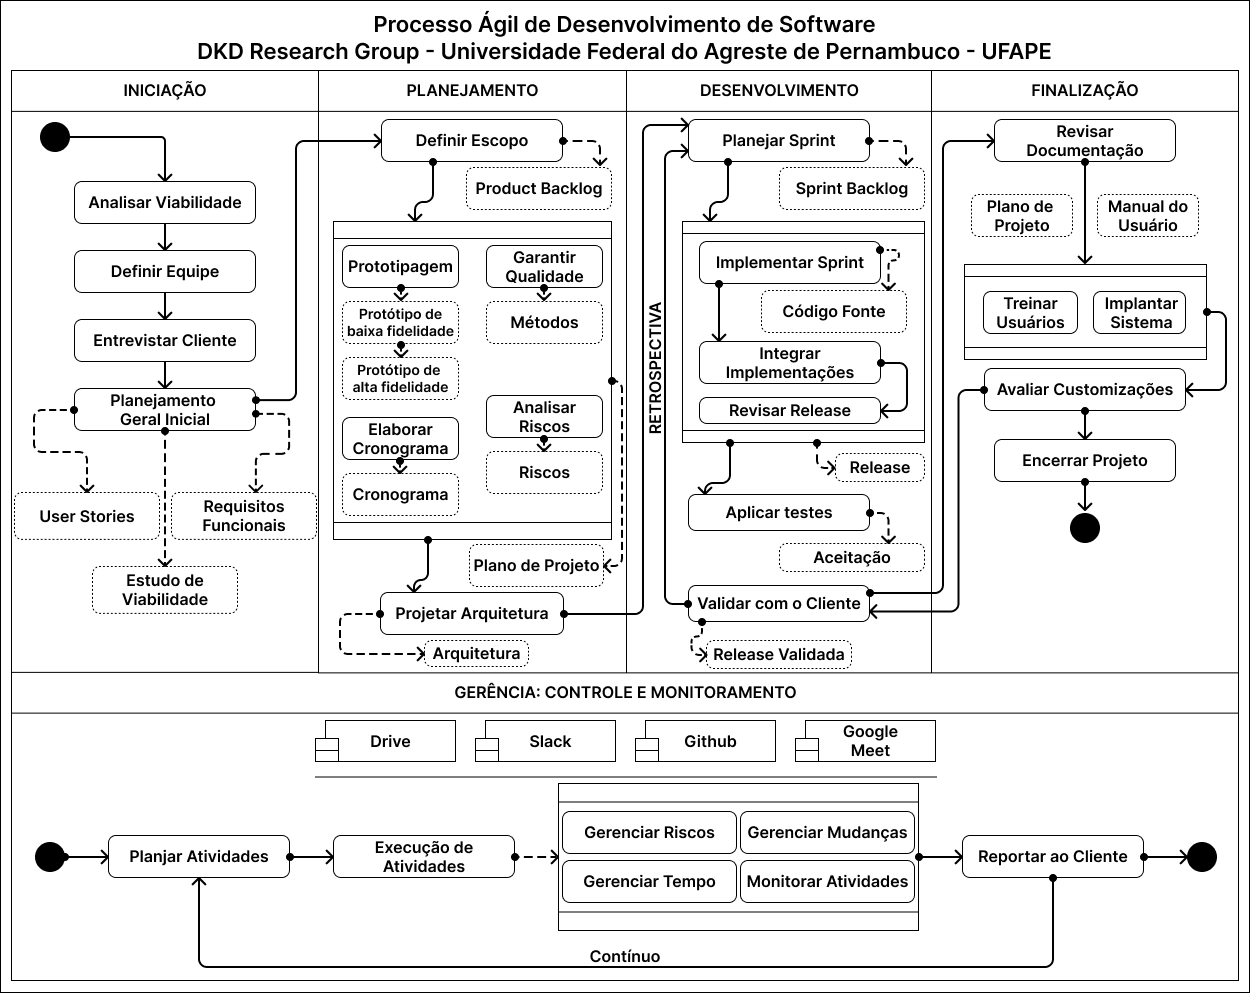
\includegraphics[width=\columnwidth]{images/processo_agil.png}
  \caption{Representação do Processo Ágil de Desenvolvimento de Software para o Enzitech}
  \acsfont{Fonte: Adaptação de DKDGroup}
  \label{fig:processo_agil}
\end{figure}

\section{Sprints}\label{sec:sprint}
Como foi explicado na seção de \nameref{ssec:metodologias_ageis}, o projeto seguiu duas metodologias que guiaram a criação do \ac{app}, o Scrum e o Kanban, muitas vezes referenciado por profissionais como "Scranban" ou algo semelhante, somente um nome genérico que aponte a junção dessas duas metodologias, portanto, o desenvolvimento do projeto foi dividido em sprints, houve um acordo entre a equipe sobre a flexibilidade das mesmas, visto que todos os envolvidos teriam que alinhar seus horários para a conclusão do projeto, ponderando entre sua vida acadêmica e profissional, o que acarretou em uma maior duração, mas não em menor desempenho ou qualidade, assim, impossibilitando manter uma sprint fixa de 2 a 4 semanas como sugerido pelo \textit{framework} Scrum. 

Como o uso do Kanban também estava presente, para a sprint ser iniciada havia um requisito: as atividades deveriam ser puxadas da coluna "TODO" na ordem de sua prioridade, portanto, com base na importância dos mesmos, tendo como foco a conclusão de um \ac{mvp}. Logo que o \ac{app} atingiu os requisitos mínimos esperados, foi gerado uma versão \textit{beta} e liberada para os usuários internos testarem, a fim de obter alguns \textit{feedbacks}.

Abaixo é possível ver uma demonstração do quadro de atividades do projeto Enzitech no Github Project\footnote{\label{githubproject}Github Project: \url{https://docs.github.com/en/issues/planning-and-tracking-with-projects/learning-about-projects/about-projects}}, plataforma utilizada como quadro adaptável, que se integra às \textit{issues} e solicitações de \textit{pull} no GitHub para ajudar no planejamento e acompanhar o projeto com eficiência.

\begin{figure}[H]
\centering
  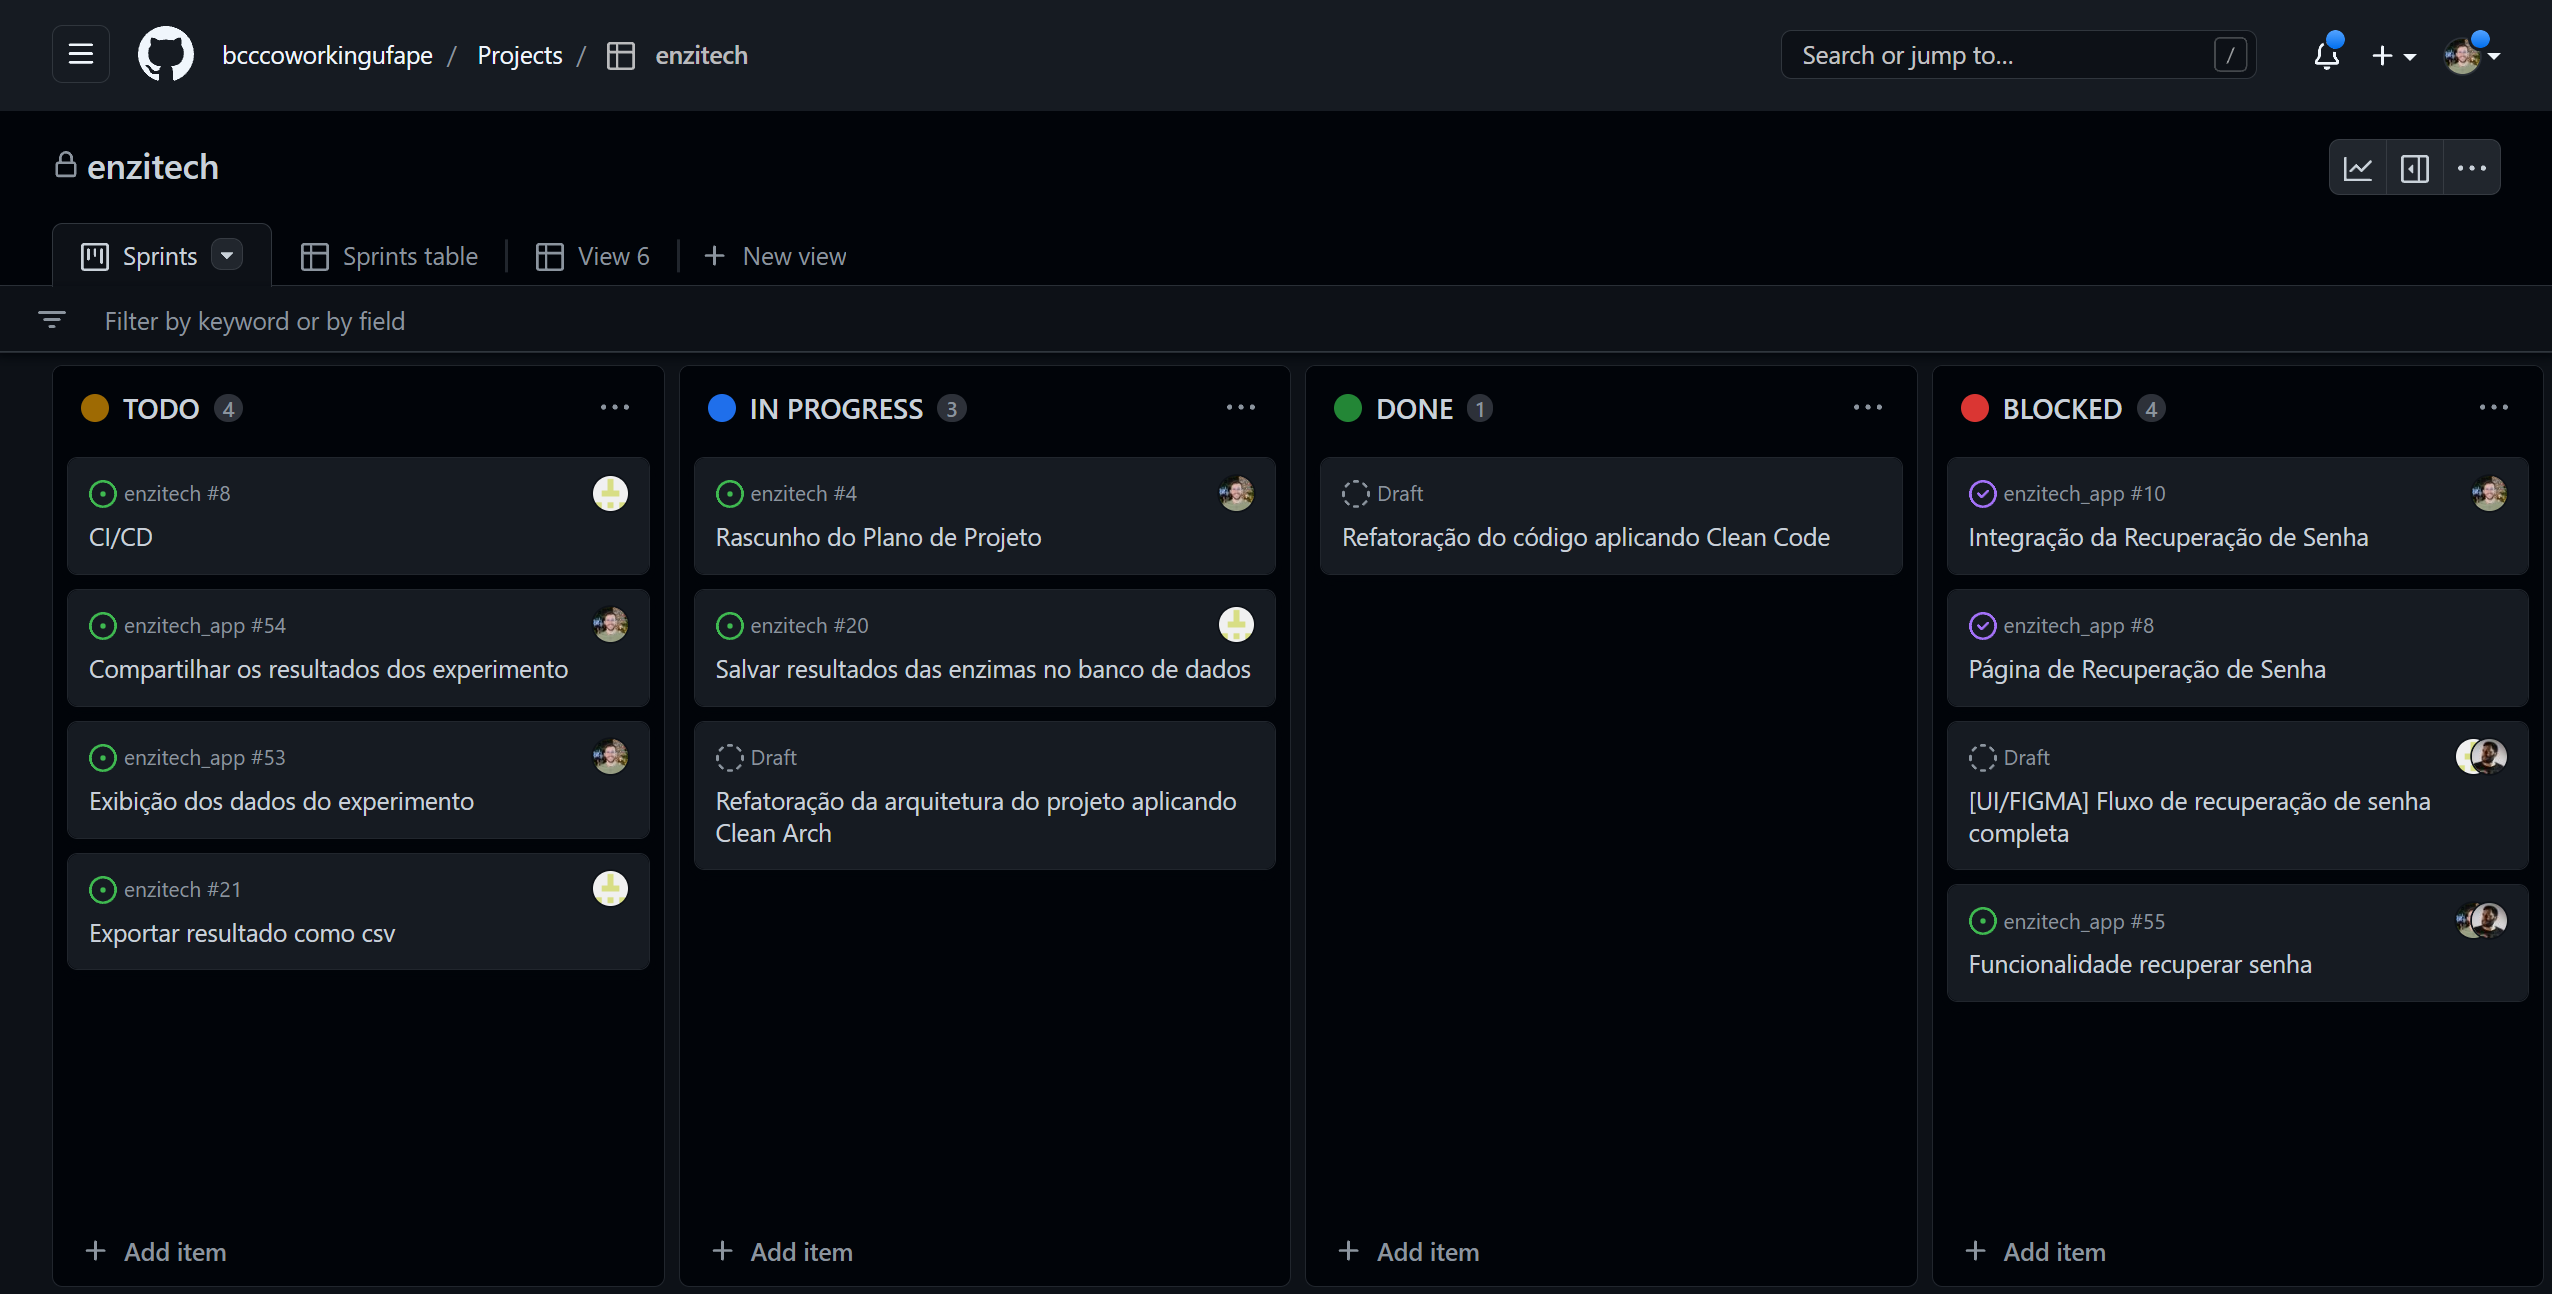
\includegraphics[width=\columnwidth]{images/quadro_projeto_github.png}
  \caption{Quadro de atividades do Enzitech no Github Project\footref{githubproject}}
  \acsfont{Fonte: Github}
  \label{fig:quadro_projeto_github}
\end{figure}

Outro dado interessante para a gestão ágil do projeto é o gráfico de eficiência e bloqueios, algo que também é disponibilizado no Github Project\footref{githubproject}, onde é possível ver o progresso do que está sendo feito para a conclusão do projeto, o fluxo de desenvolvimento e as mudanças de escopo ao longo do tempo. Sendo possível identificar gargalos e problemas que impedem o progresso da equipe. Abaixo está um exemplo do gráfico do projeto.

\begin{figure}[H]
\centering
  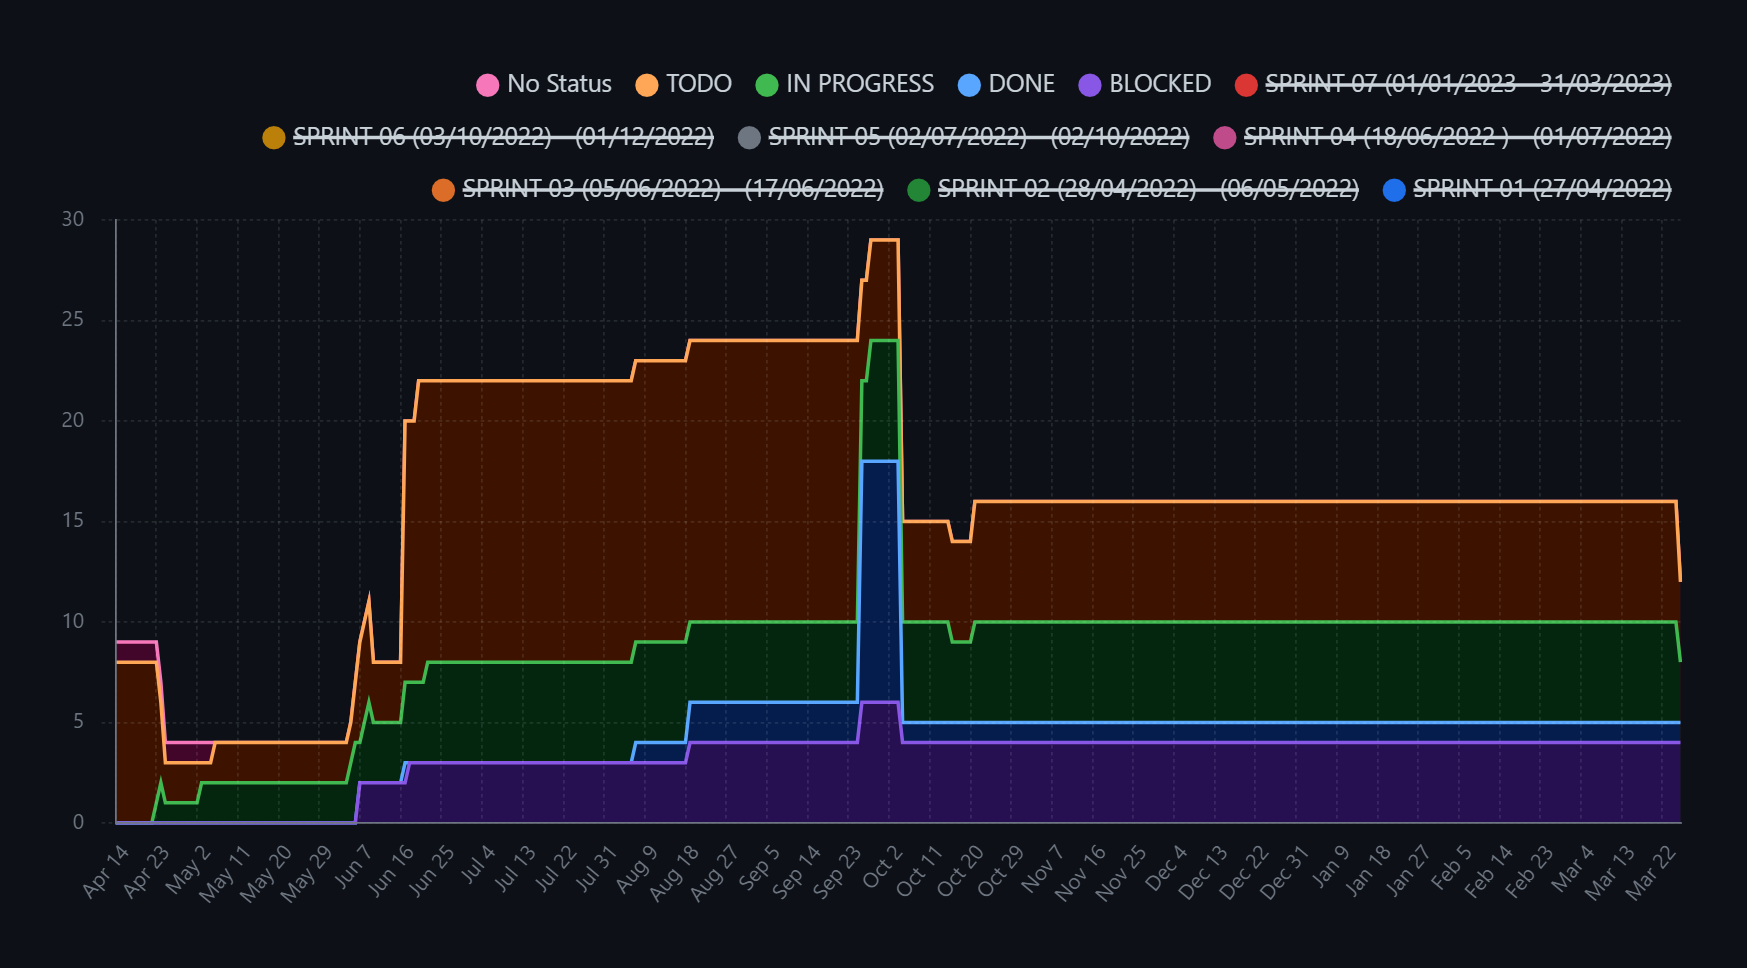
\includegraphics[width=\columnwidth]{images/grafico_projeto_github.png}
  \caption{Gráfico de \textit{Burn Up} das atividades do Enzitech no Github Project\footref{githubproject}}
  \acsfont{Fonte: Github}
  \label{fig:grafico_projeto_github}
\end{figure}

A seguir serão explicadas brevemente o planejamento, desenvolvimento e resultados obtidos em cada sprint.

% \subsection{Sprint 1}\label{ssec:sprint1}

% \subsubsection{Planejamento}\label{sssec:planejamento1}
Para a primeira sprint, foi planejado o estudo da última versão do protótipo, o desenvolvimento da identidade visual do \ac{app}, incluindo seu ícone/logotipo, o \textit{back-end} tratou de desenvolver o \ac{crud} de usuários, assim como a documentação da \ac{api} que seria acessada pelo \textit{front-end(mobile)}, além disso, houve a configuração inicial dos bancos de dados e servidores para os ambientes de teste e desenvolvimento.

Simultaneamente, houve um estudo para decidir qual arquitetura seria adotada no \ac{app}, seu sistema de gerenciamento de estado e outros detalhes técnicos, como a criação do arquivo de \textit{design-system} para o \ac{app}. 

Nesta primeira sprint não houveram muitos impedimentos, e tudo fluiu dentro do esperado, levando em consideração que o projeto estava sendo criado e configurado ainda dentro deste período.
% \subsubsection{Desenvolvimento}\label{sssec:desenvolvimento1}
% Como será explicada numa seção mais detalhada a frente, o padrão arquitetural escolhido foi o \ac{mvvm}
% \subsubsection{Resultados}\label{sssec:resultados1}

% \subsection{Sprint 2}\label{ssec:sprint2}
Na segunda sprint foi iniciado o desenvolvimento da tela de \textit{home}, ainda sem integrações, somente para alinhar a estrutura do projeto com a arquitetura inicialmente escolhida, o \ac{mvvm}, um padrão de arquitetura em \textit{software} que facilita a separação do desenvolvimento da \ac{ui} – em português, Interface Gráfica do Usuário – do desenvolvimento da lógica de negócios ou lógica de \textit{back-end} (o \textit{model}), de modo que a \textit{view} não dependa de nenhuma plataforma de modelo específica.

\begin{figure}[H]
\centering
  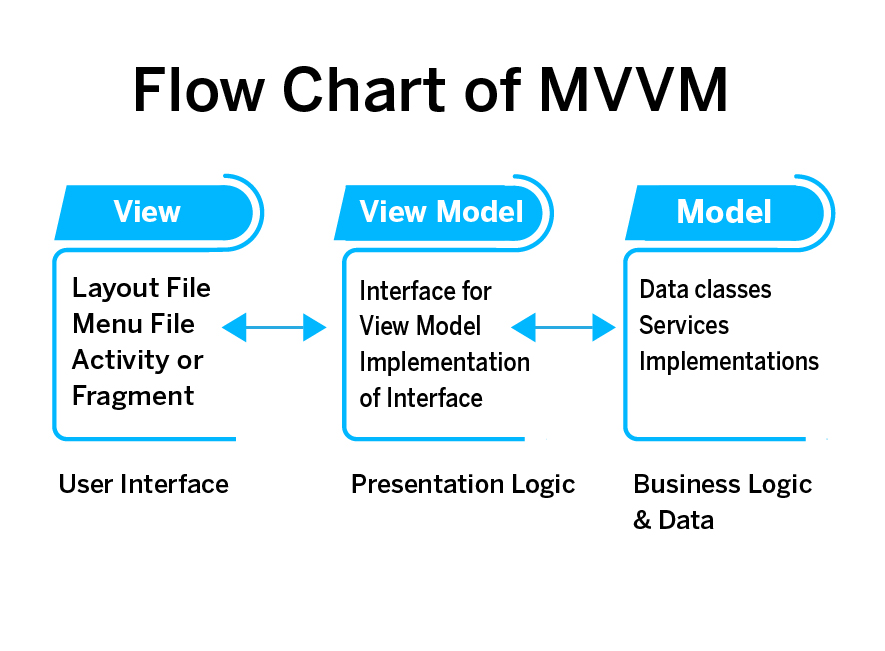
\includegraphics[width=\columnwidth/2]{images/MVVM-architecture.jpg}
  \caption{Descrição do padrão \ac{mvvm}}
  \acsfont{Fonte: \cite{appventurez}}
  \label{fig:MVVM-architecture}
\end{figure}

Além disso, foi desenvolvido a classe para requisições \ac{http} no \ac{app}, como também, mais telas foram desenhadas no protótipo de alta fidelidade. Ao fim, foi possível ter uma primeira versão executável do projeto, o qual já estava apto a se conectar à \textit{Web} e fazer requisições na \ac{api} que estava sendo desenvolvida em paralelo. 

% \subsection{Sprint 3}\label{ssec:sprint3}
Os objetivos da terceira sprint foram implementar as telas e realizar as integrações dos \textit{endpoints} desenvolvidos para a \ac{api}, portanto, como resultado, foram contempladas os seguintes requisitos funcionais:
\begin{itemize}
   \item RF01 - Cadastro de usuário;
   \item RF02 - \textit{Login};
   \item RF03 - Recuperação de senha;
   \item RF12 - Listagem de experimentos;
 \end{itemize}

Ademais, o desenvolvimento do protótipo seguiu avançando e correções no código e na estrutura do \ac{app} foram realizadas, atingindo a seguinte estrutura:
\begin{figure}[H]
\centering
  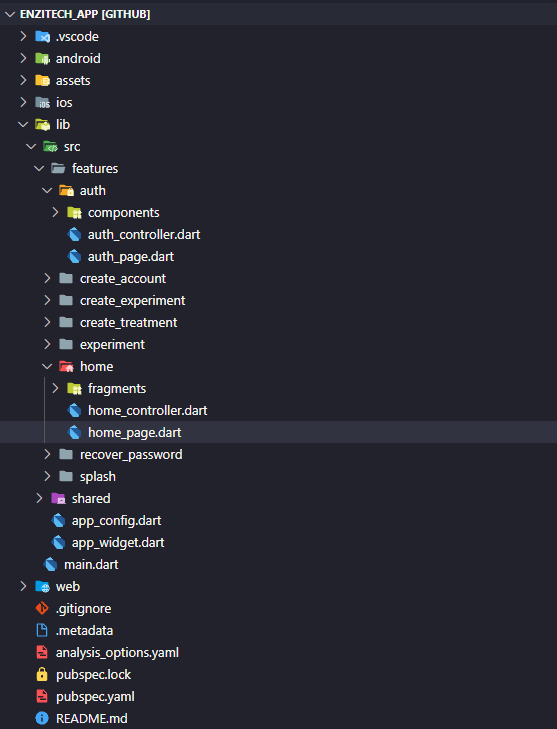
\includegraphics[width=\columnwidth/2]{images/app_sprint_3.png}
  \caption{Estrutura do projeto ao fim da terceira sprint}
  \acsfont{Fonte: Autoria própria}
  \label{fig:app_sprint_3}
\end{figure}

Outro ponto importante é que neste momento já foram adicionadas algumas dependências ao projeto que facilitaram o desenvolvimento, entre elas, é válido destacar as seguintes:
\begin{itemize}
   \item \textit{dio}: Biblioteca utilizada para realizar requisições \ac{http};
   \item \textit{provider}: Biblioteca utilizada para lidar com o gerenciamento de estado do \ac{app};
   \item \textit{shared\_preferences}: Biblioteca utilizada para armazenar dados simples de forma persistente no dispositivo;
 \end{itemize}

No fim deste arquivo, na seção de Apêndice, em "\nameref{code:home-sprint3}", um trecho da \textit{view} de \textit{Home Page} desenvolvida até este ponto está disponível.

Desta forma, adiantando a estrutura para as próximas \textit{features} a serem implementadas e obtendo como resultado um \ac{app} que já tomava o formato desejado, assim, entregando valor com a conclusão da sprint.

% \subsection{Sprint 4}\label{ssec:sprint4}
Já na quarta sprint, os objetivos foram as implementações das telas e integrações dos \textit{endpoints} desenvolvidos que restavam, abrangindo os seguintes requisitos funcionais:
\begin{itemize}
   \item RF04 - Cadastro de tratamento;
   \item RF06 - Listagem de tratamentos;
   \item RF07 - Cadastro de enzima;
   \item RF09 - Listagem de enzimas;
   \item RF10 - Criação de experimento;
 \end{itemize}

 Neste ponto, o \ac{app} já possuía as principais \textit{features} para seguir com a parte de experimentos e cálculos, alguns testes foram realizados para verificar o fluxo de informações entre as telas e se tudo estava integrado corretamente, apesar do projeto ser desenvolvido para multiplataformas, vale salientar que inicialmente o \ac{app} só estará disponível para o sistema Android, visto que a publicação de \acp{app} neste sistema é muito mais simples e barata se comparada a \acp{app} para iOS, cuja licença para publicar \acp{app} na loja custa um valor considerável. Não é descartada a hipótese de lançar o \ac{app} para dispositivos iOS no futuro, contanto que exista demanda dos usuários para tal.

 O projeto necessitou de uma configuração no \textit{Firebase} \footnote{\label{firebase}\textit{Firebase}: \url{https://firebase.google.com/}} para o lançamento de versões internas para teste no \textit{App Distribution}, o que foi realizado aqui nesta sprint, com isso, foi possível escolher alguns usuários envolvidos no projeto para realizarem os testes, instalando o mesmo em seus dispositivos pessoais. 

 Abaixo, na \figref{fig:app_distribution}, uma demonstração do painel do \textit{App Distribution} para o \ac{app}, para utilizar este serviço foi preciso integrar o Firebase SDK no \ac{app} Flutter e configurar o processo de build para enviar o \textsc{.apk} ou \textsc{.aab} (versões compiladas para o Android) para o Firebase. Em seguida, foi necessário criar um grupo de testadores e conceder acesso ao \ac{app}.

Os testadores receberam um convite por e-mail com um link para fazer o download do \ac{app} e começar a testá-lo. No painel, é possível controlar quem tem acesso às versões do \ac{app}, permitindo que apenas usuários específicos o baixem e o testem, uma vez que ele tenha sido distribuído, é possível monitorar as métricas de uso e coletar feedback dos testadores, o que ajuda a melhorar o produto antes de lançá-lo oficialmente.

\begin{figure}[H]
\centering
  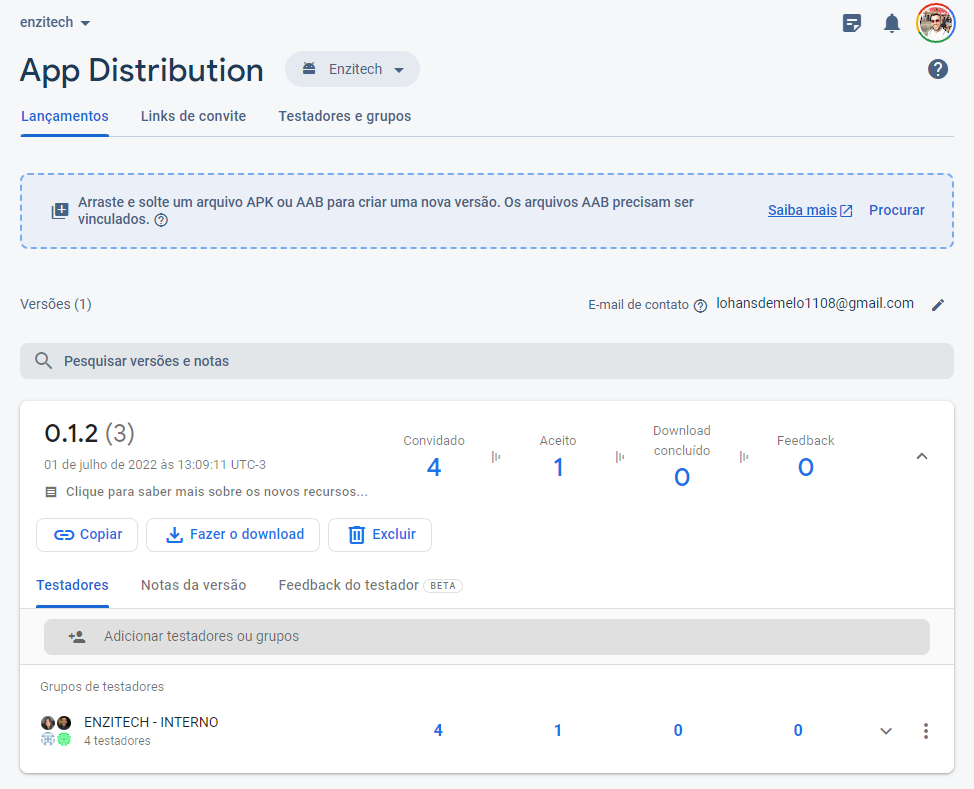
\includegraphics[width=\columnwidth]{images/app_distribution.png}
  \caption{Aba do \textit{Firebase App Distribution} do projeto Enzitech}
  \acsfont{Fonte: \textit{Firebase}\footref{firebase}}
  \label{fig:app_distribution}
\end{figure}
 
% \subsection{Sprint 5}\label{ssec:sprint5}
Na quita sprint, o protótipo de alta fidelidade atingiu a maturidade que o projeto necessitava, desta forma o foco de desenvolvimento foi voltado para as implementações das \textit{features} de deletar as entidades que já eram possíveis serem criadas, desta forma, os seguintes requisitos funcionais foram concluídos:
\begin{itemize}
   \item RF05 - Deletar um tratamento;
   \item RF08 - Deletar uma enzima;
   \item RF11 - Deletar um experimento;
   \item RF13 - Utilizar filtros na listagem de experimentos;
 \end{itemize}

A RF13 foi iniciada nesta sprint, mas não foi concluída, pois a história foi dividida em duas \textit{spikes} — a definição de \textit{"Spike"} vem do \textit{Extreme Programming} e surgiu a partir da \textit{"Spike Solution"}, que é um programa ou protótipo funcional usado para explorar possíveis soluções para um problema específico — uma para o desenvolvimento de um \textit{switch} entre experimentos concluídos e em andamento e outra para o desenvolvimento do filtro por ordenação de características de um experimento, portanto, nessa, o \textit{switch} foi implementado, porém sem integrações com a \ac{api} ainda.

Nesta sprint mais requisitos foram concluídos, houveram vários ajustes e correções de \textit{bugs}, como os de fluxos após criação de um experimento, junto disso houveram alguns estudos para uma futura refatoração que será abordada na última sprint, foi notado que o escopo do projeto precisaria de uma arquitetura mais refinada, logo, este tempo foi reservado para estudo junto ao desenvolvimento.  
 
% \subsection{Sprint 6}\label{ssec:sprint6}
Nesta sexta sprint, os seguintes requisitos funcionais foram atacados:
\begin{itemize}
   \item RF13 - Utilizar filtros na listagem de experimentos;
   \item RF14 - Visualizar detalhes de um experimento;
   \item RF15 - Inserção de dados para o cálculo enzimático no experimento;
 \end{itemize}

Na \figref{fig:filtros_sprint_6} é possível ver o \textit{dialog} desenvolvido para a escolha de filtros na listagem de experimentos, nele é possível escolher a ordenação por ordem crescente ou decrescente, assim como, é possível mudar a ordenação de acordo com o nome, descrição, repetições, progresso, data de criação ou data de modificação. Desta forma, finalizando o requisito funcional 13 por completo.
 
 \begin{figure}[H]
\centering
  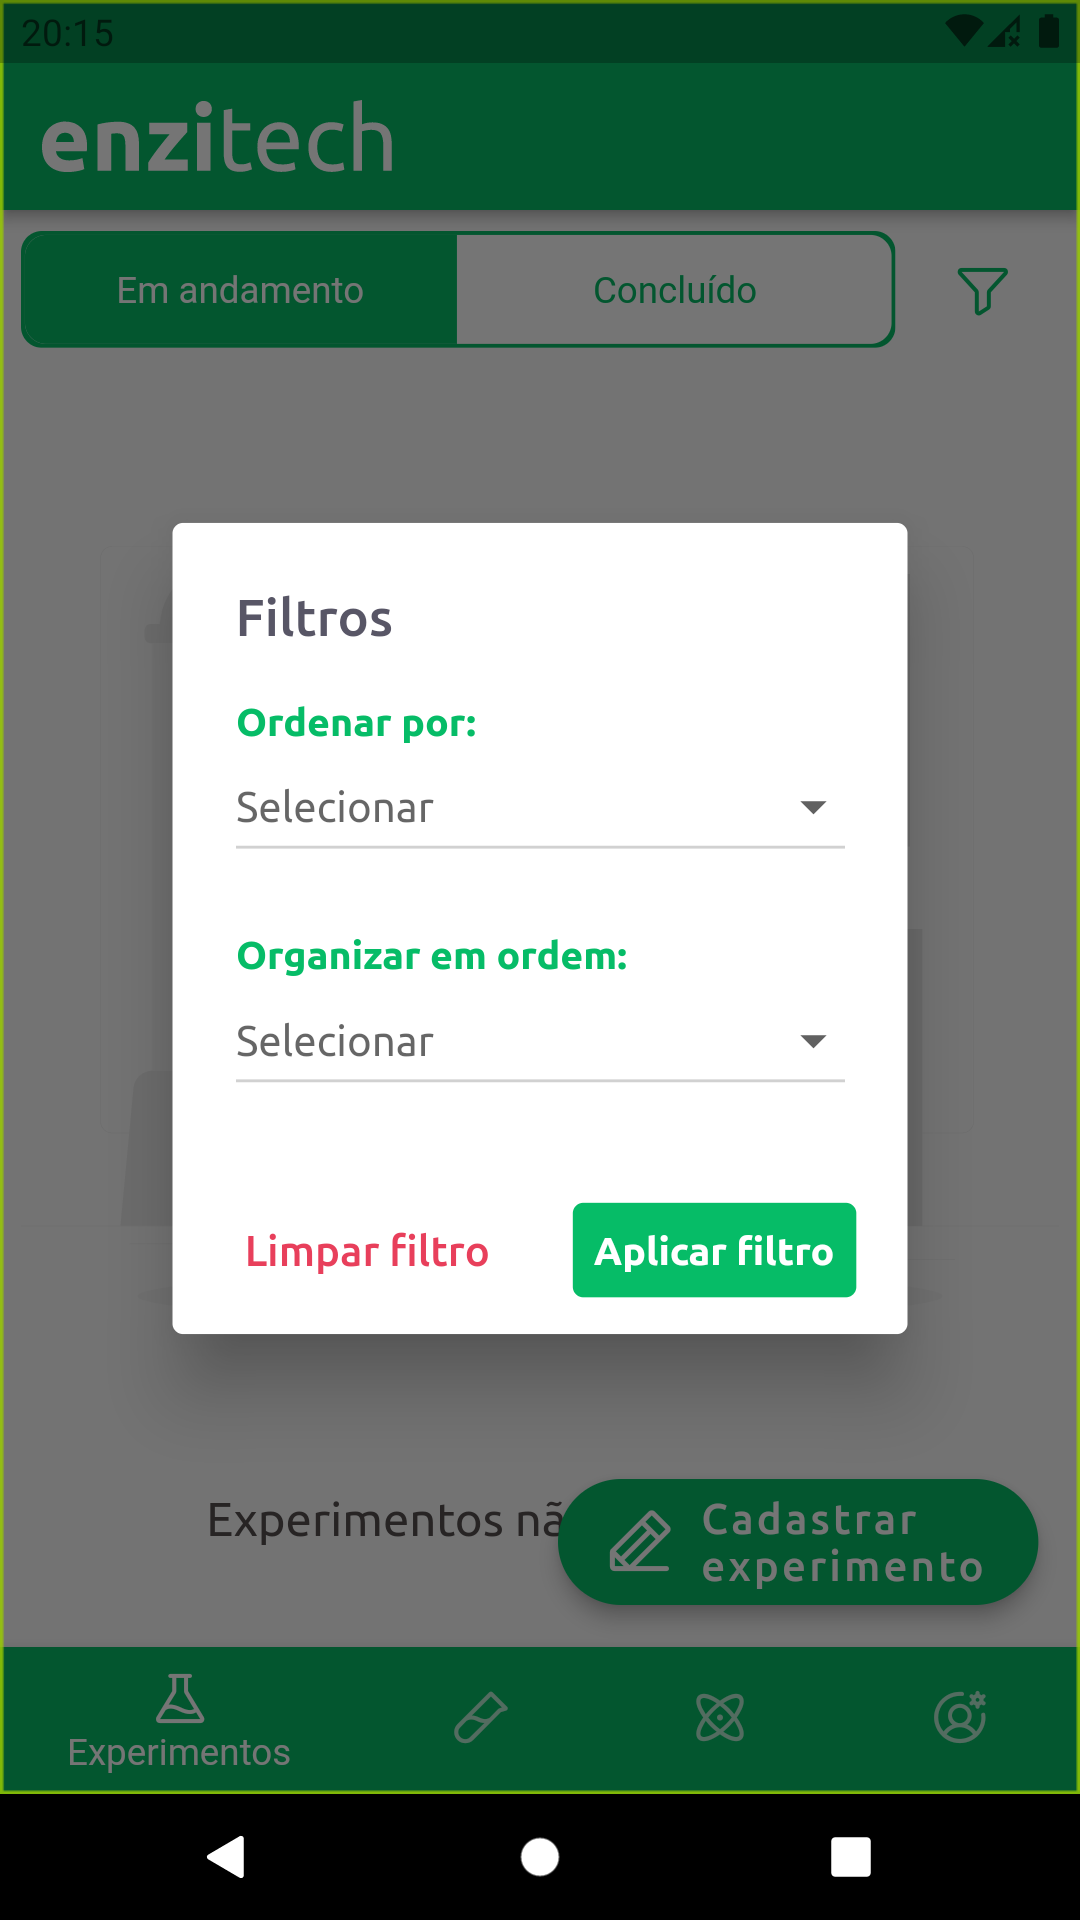
\includegraphics[width=\columnwidth/2]{images/filtros_sprint_6.png}
  \caption{Filtros de experimento do Enzitech}
  \acsfont{Fonte: Autoria própria}
  \label{fig:filtros_sprint_6}
\end{figure}

Aqui também foi desenvolvido todo o fluxo para visualização dos detalhes de um experimento, o que dá acesso às opções de inserir dados e visualizar os mesmos. Nesta sprint também foi aplicado um estudo de performance feito no \ac{app}, o qual até este momento só carregava os dados após a \textit{splashscreen} (tela antes da home/listagem de experimentos), o que não era o melhor cenário possível, então, após alguns artigos lidos e estudos de caso, a solução encontrada foi de fazer a primeira carga de informações do Enzitech ao \ac{app} ser aberto, ou seja, em sua inicialização, de forma assíncrona, onde, se preciso fosse, a tela de \textit{splashscreen} faria sua responsabilidade, que é de segurar a navegação do usuário até que todos os dados estejam preparados para o uso. 

Desta forma, houve um ganho de performance que diminuiu o tempo de carregamento do \ac{app}, trazendo uma sensação de maior fluidez.

Como podemos ver no Código Fonte \nameref{code:check-auth} o sistema primeiro checa se há algum \textit{token} de autenticação guardado, caso negativo ele segue da \textit{splashscreen} de volta para a tela de \textit{login} para o usuário realizar a autenticação novamente, caso positivo a navegação segue, os dados são pré-carregados e logo após o usuário é levado para a tela inicial do Enzitech.

Além disso, foi implementado uma \textit{feature} para lidar com ações sensíveis, como a de exclusão de itens, desta forma, é possível ativar ou desativar nas configurações do \ac{app} um alerta de confirmação de exclusão de experimentos, tratamentos e enzimas, o qual, além deste passo de segurança implementado, oferece outra funcionalidade, independente desta anterior estar ativada ou não, que é a de desfazer ações destrutivas, ou seja, o usuário pode se arrepender da exclusão (ou tê-la feito por engano) e recuperar esta informação, assim, oferecendo um passo de segurança a mais para os dados, abaixo na \figref{fig:fluxo_exclusao} é possível ver sua aplicação em um tratamento.

\begin{figure}[H]

\centering
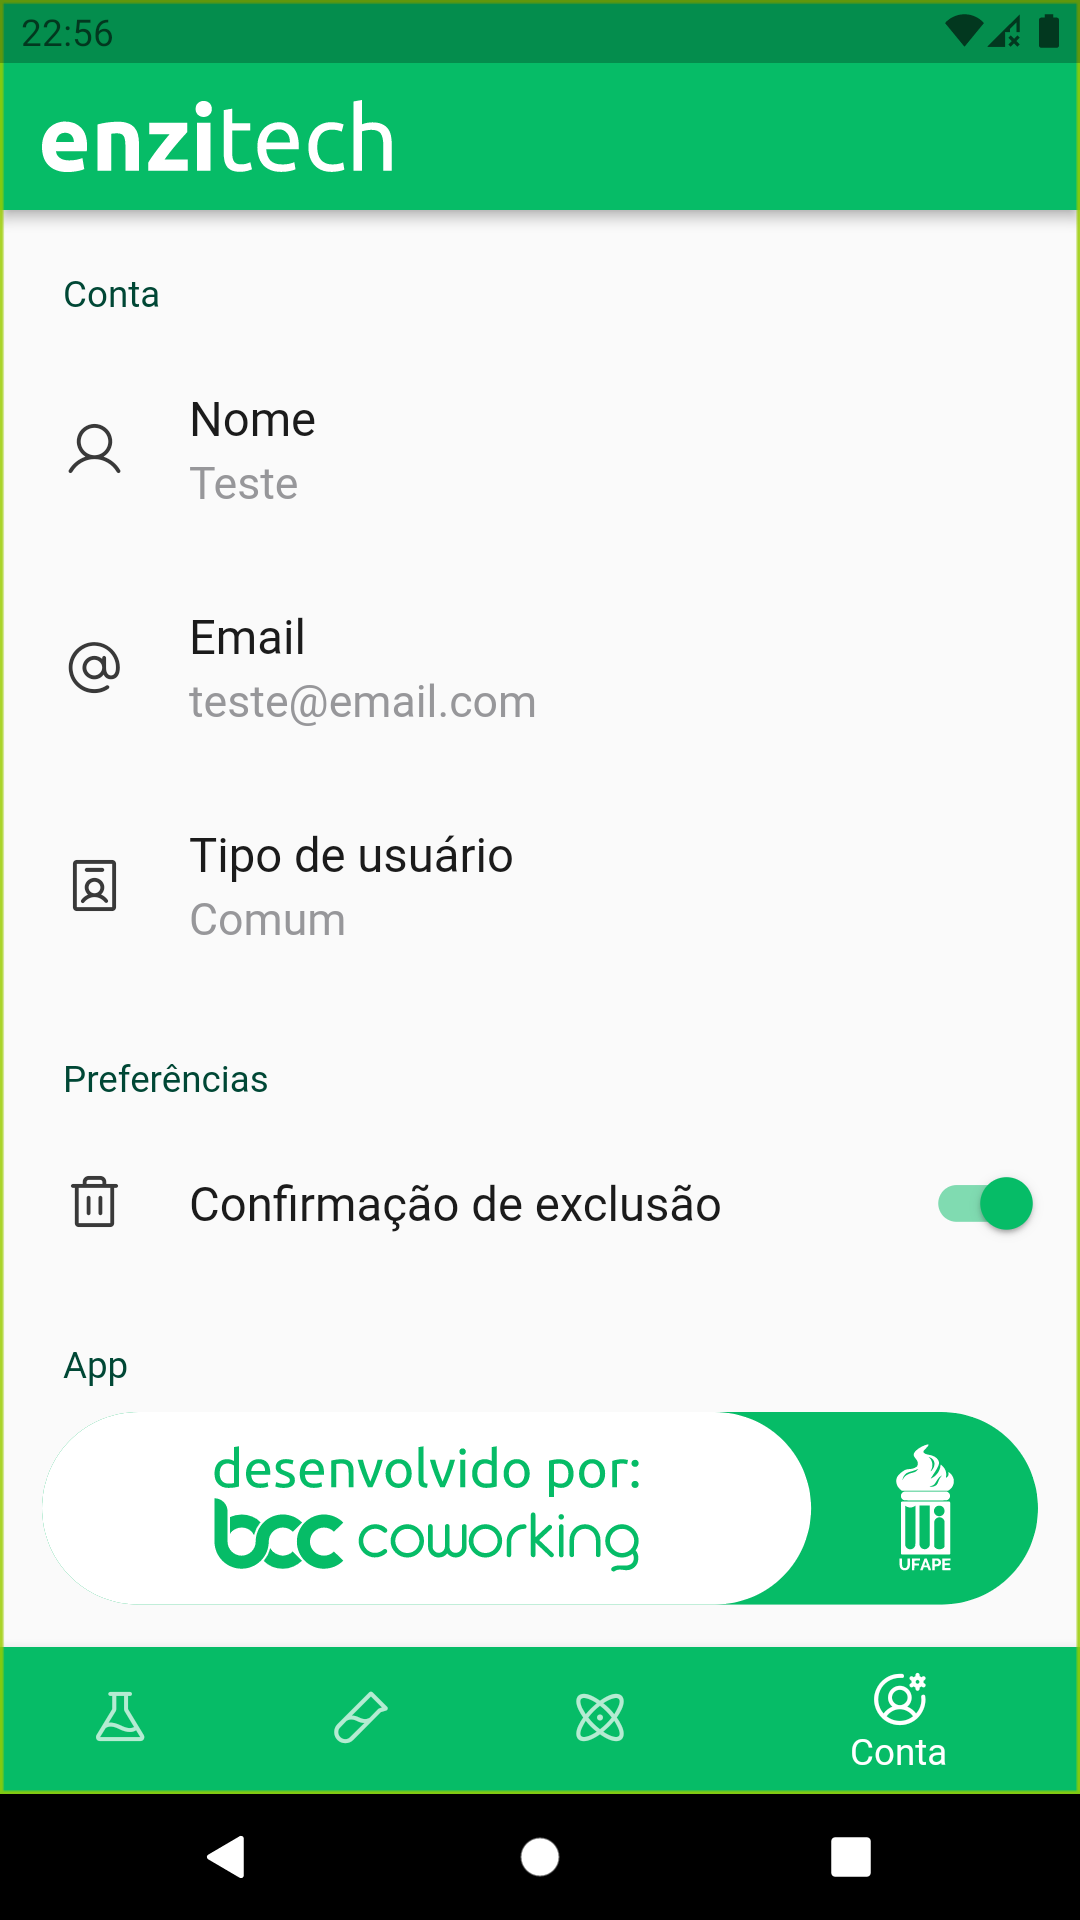
\includegraphics[width=.3\textwidth]{images/exclusao_1_sprint_6.png}\hfill
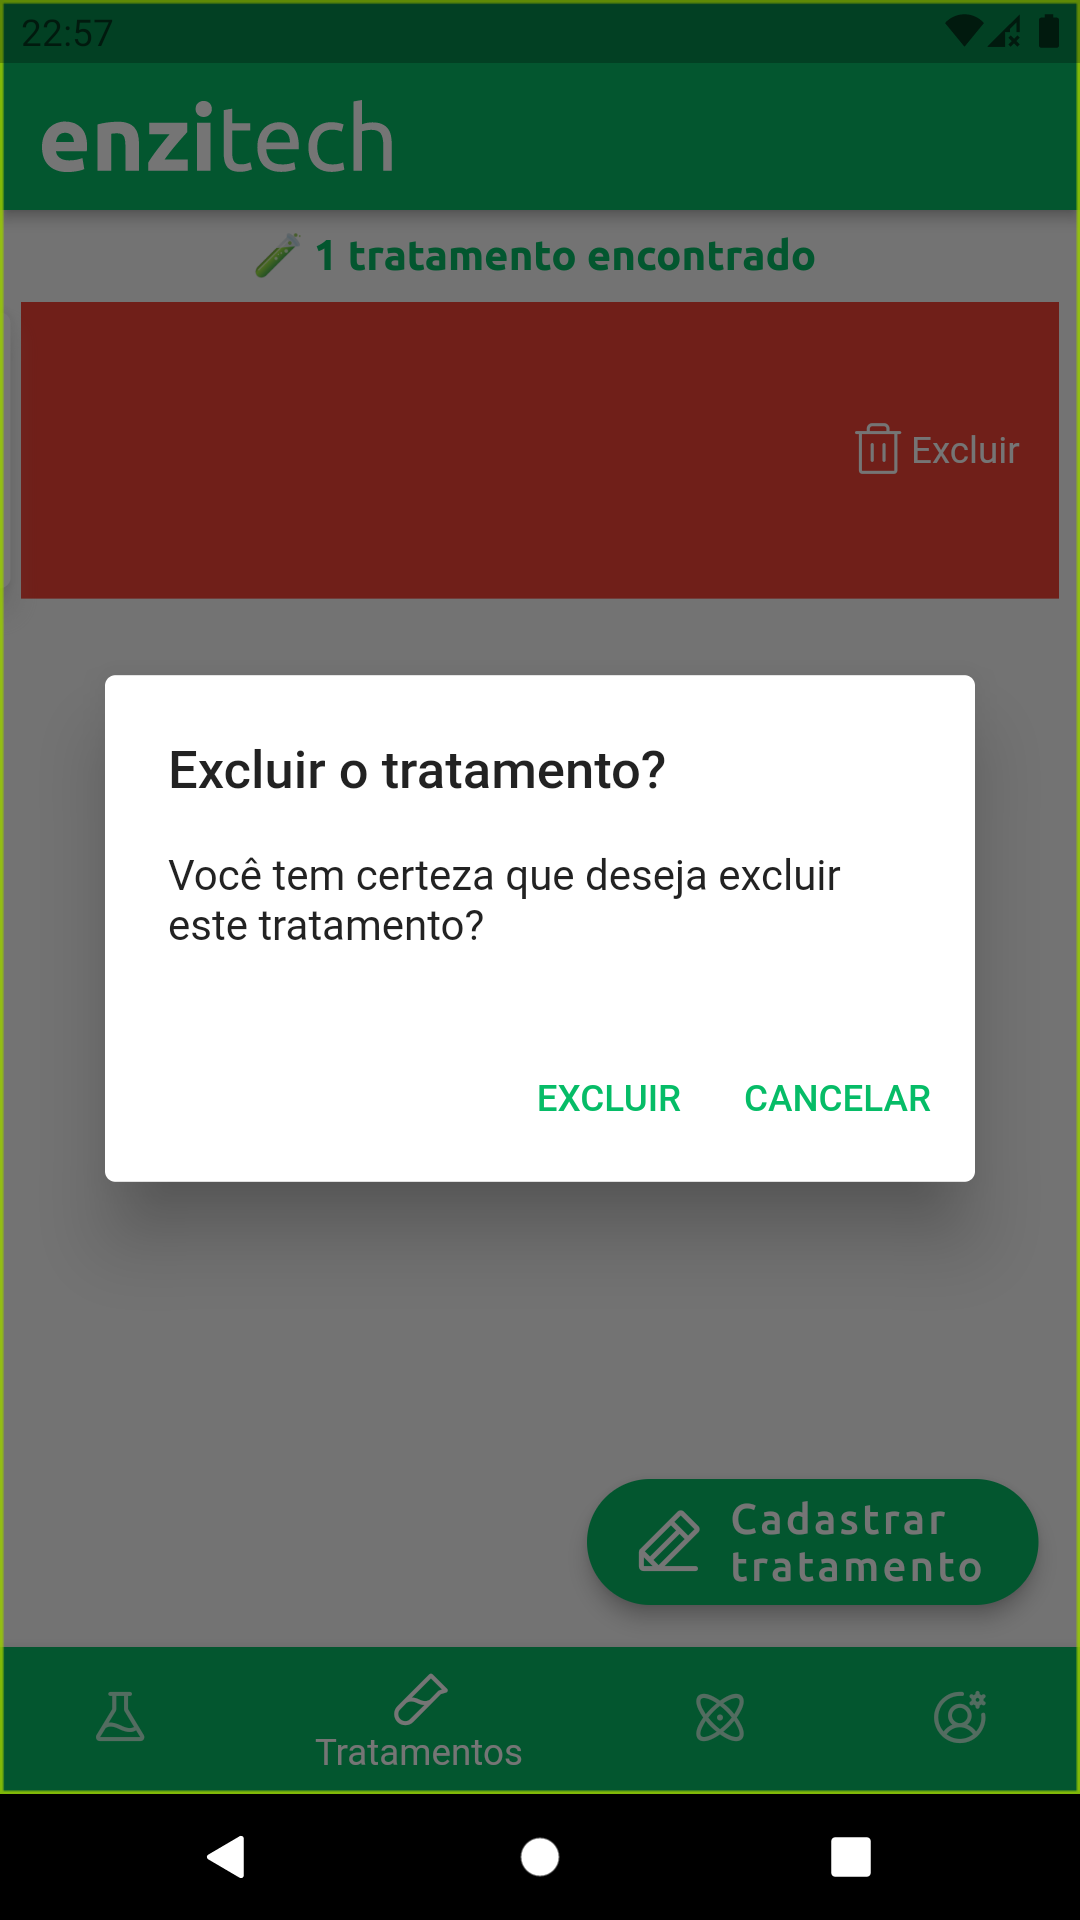
\includegraphics[width=.3\textwidth]{images/exclusao_2_sprint_6.png}\hfill
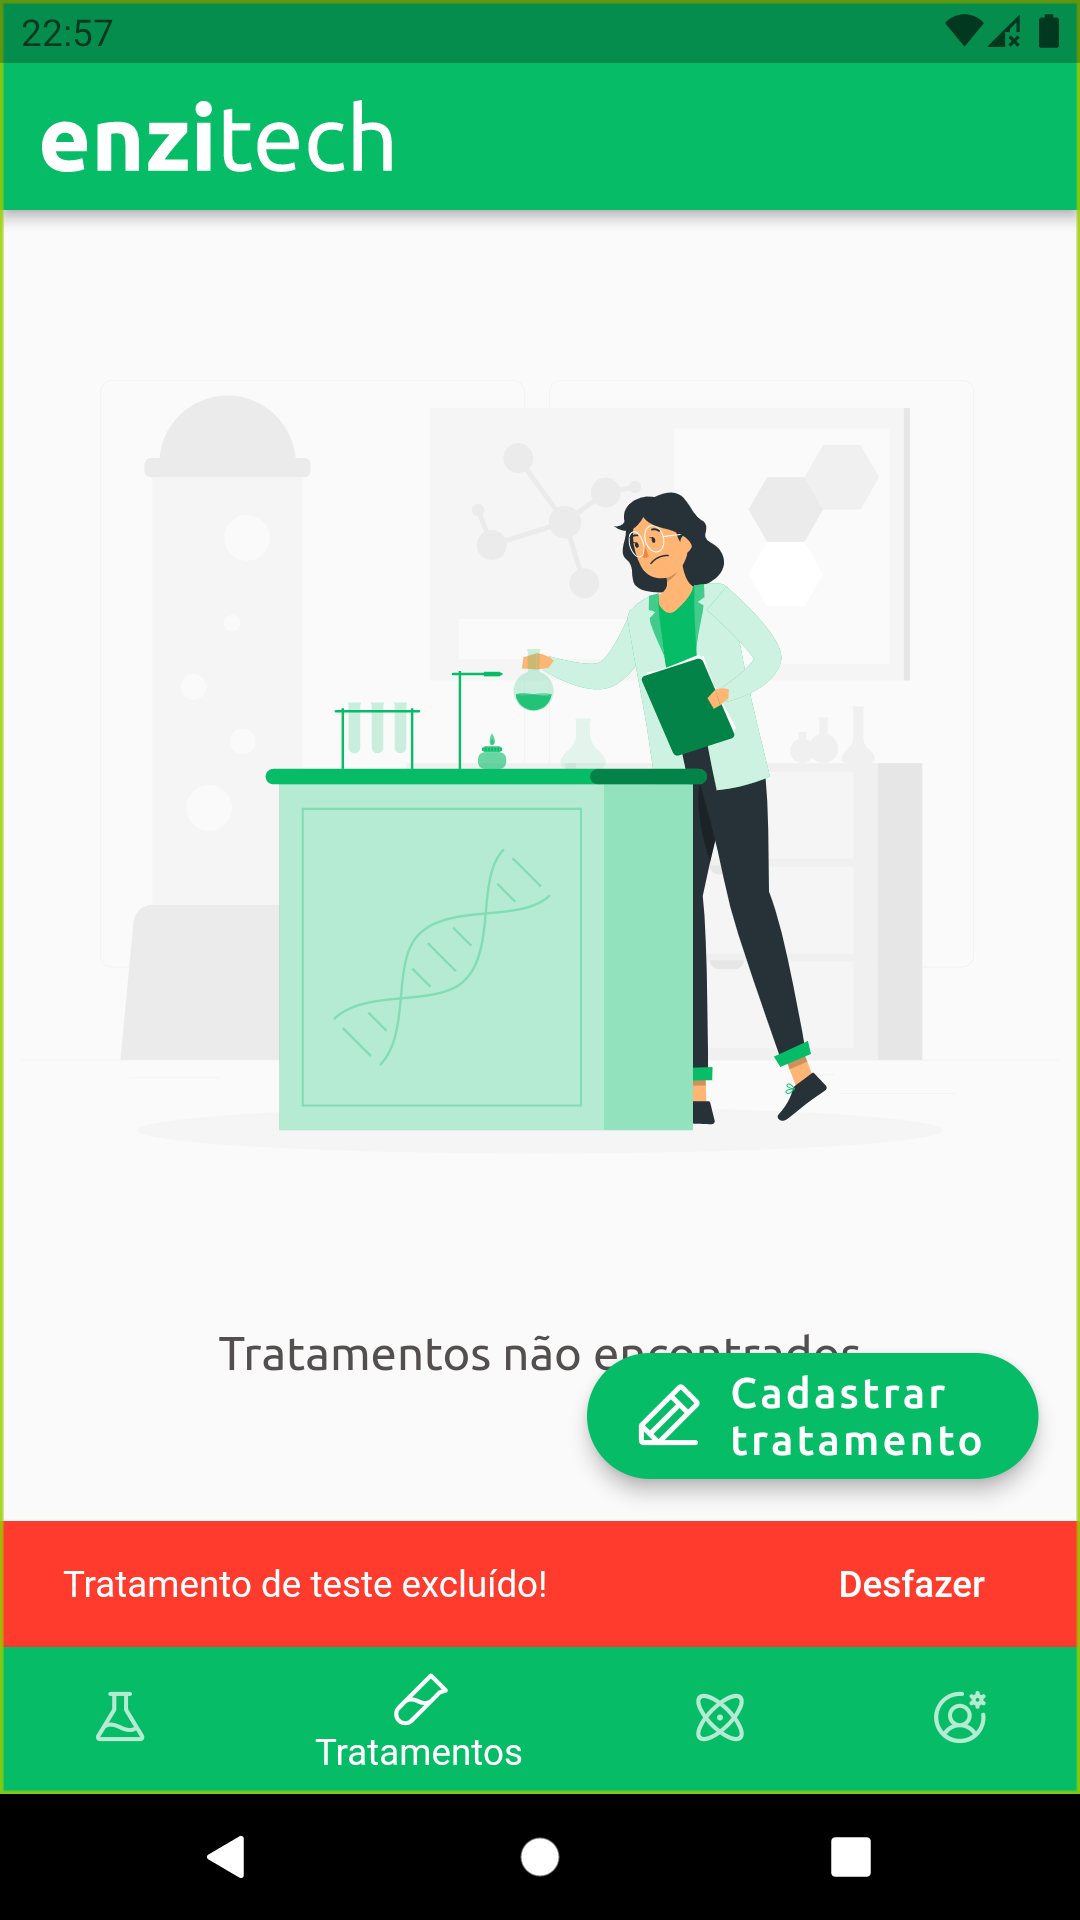
\includegraphics[width=.3\textwidth]{images/exclusao_3_sprint_6.png}

\caption{Fluxo de exclusão de um tratamento com a opção de confirmação de exclusão ativada}
\label{fig:fluxo_exclusao}

\end{figure}

% \subsection{Sprint 7}\label{ssec:sprint7}
Na sétima e última sprint do projeto o projeto houve uma enorme refatoração de arquitetura, como comentado anteriormente, aqui, além dessa refatoração que não adiciona funcionalidades, mas garante a estabilidade do \ac{app} e permite que o mesmo possa receber novas funcionalidades de forma mais fácil e sem problemas, houve a conclusão dos requisitos funcionais restantes, são eles:
\begin{itemize}
   \item RF16 - Visualização de resultados discrepantes do cálculo enzimático antes de salvar no experimento;
   \item RF17 - Edição de resultados discrepantes do cálculo enzimático antes de salvar no experimento;
   \item RF18 - Opção de salvar os resultados do cálculo enzimático no experimento;
   \item RF19 - Visualização de todos os resultados e o progresso do experimento;
   \item RF20 - Exportação dos resultados do experimento;
 \end{itemize}

 Nesta refatoração foi aplicado o conceito de Arquitetura Limpa proposto pelo Uncle Bob, que já foi explicado no capítulo de \nameref{chp:teoria} e será aprofundada na seção \nameref{sec:arquitetura} deste capítulo, assim como houve a troca de alguns pacotes do aplicativo, portanto, com a aplicação da arquitetura limpa, foi possível isolar os pacotes adicionados ao projeto utilizando contratos/interfaces para abstrair sua implementação, permitindo uma troca mais fácil, caso necessário, no futuro... A estrutura do projeto ficou da seguinte forma:

 \begin{figure}[H]
\centering
  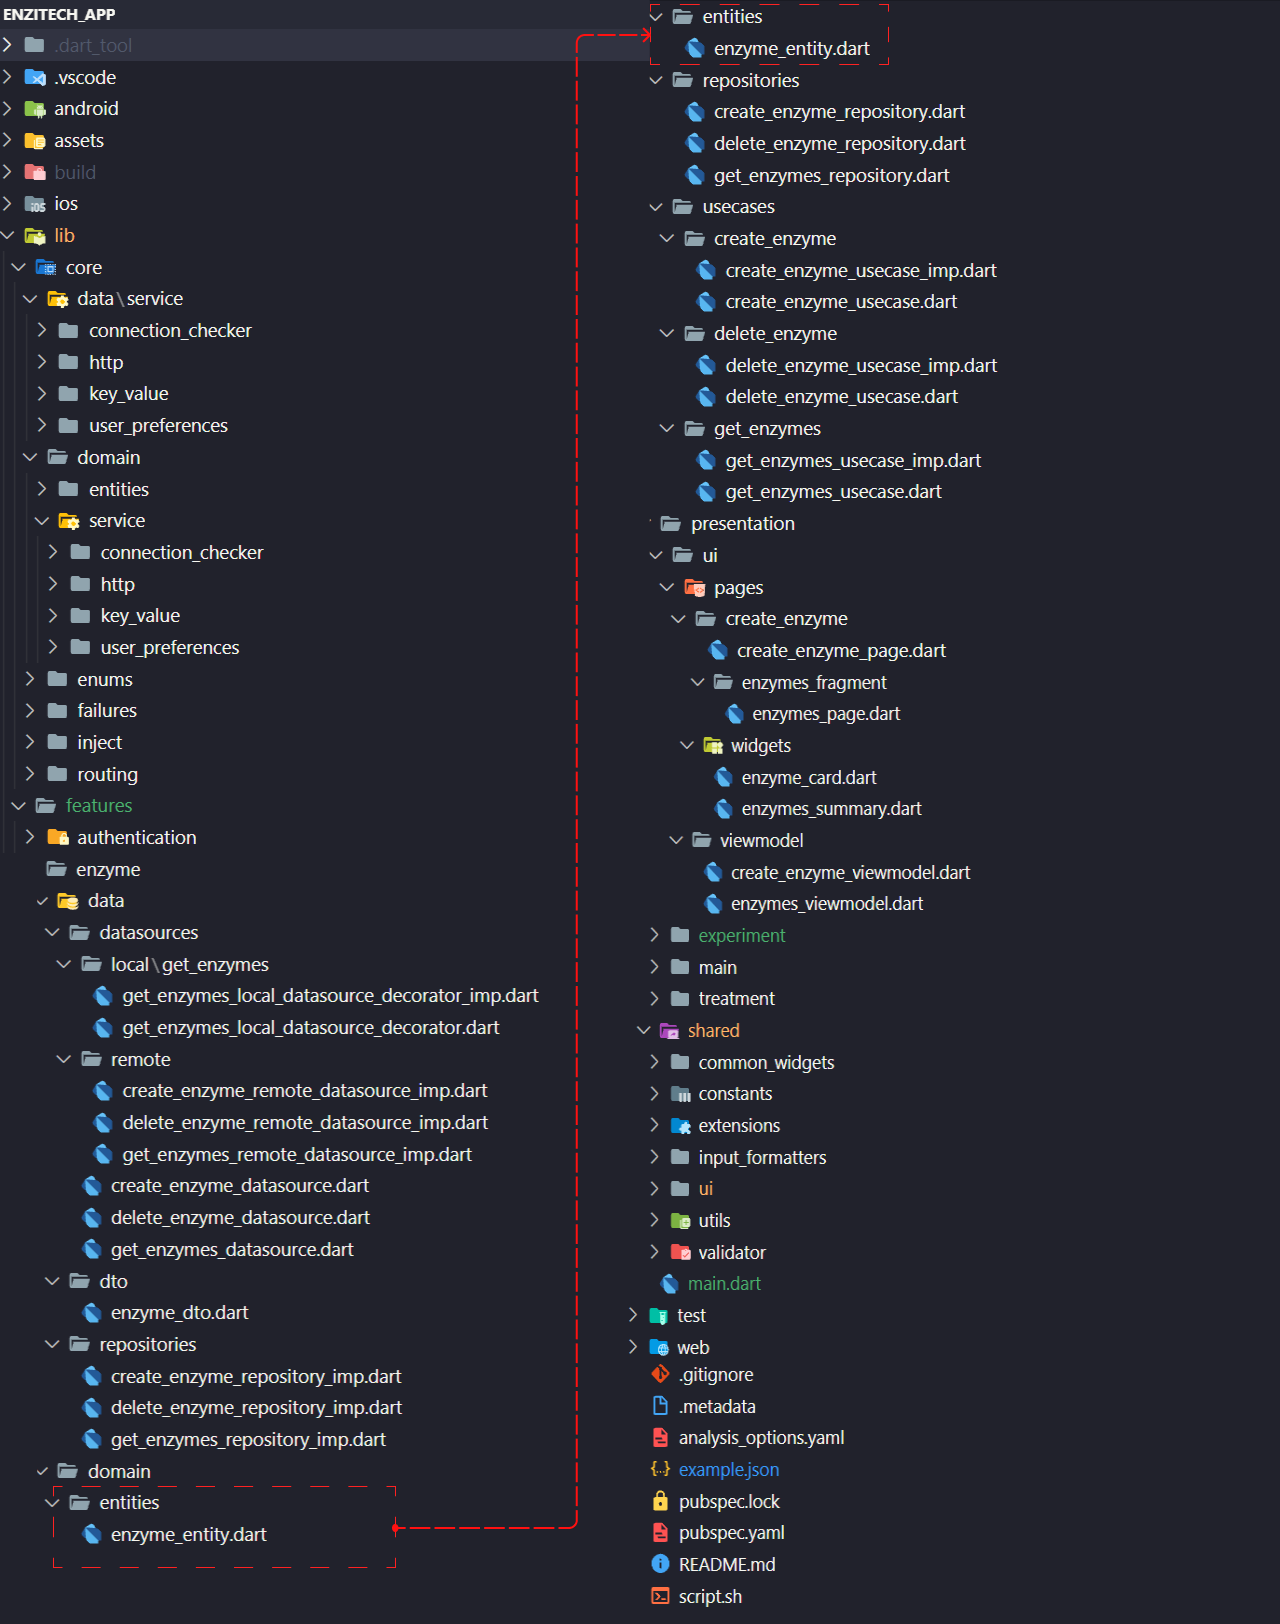
\includegraphics[width=0.85\columnwidth]{images/estrutura_app_final.png}
  \caption{Estrutura final do aplicativo em Flutter para o Enzitech}
  \acsfont{Fonte: Autoria própria}
  \label{fig:estrutura_app_final}
\end{figure}

Sintetizando toda essa estrutura, temos a separação dos requisitos funcionais baseadas em \textit{features}, como mostrado na \figref{fig:estrutura_app_final}, tudo relacionado a enzimas no aplicativo está na \textit{feature "enzyme"}, são elas: as telas, \textit{widgets} e os \textit{ViewModels} de cadastrar, deletar e obter listagem das enzimas, isto para a camada de \textit{Presentation}, seguindo o que a arquitetura exige, na camada de \textit{Domain} estão as entidades, interfaces e implementações dos Casos de Uso e a interface para os Repositórios, por fim, na camada de \textit{Data} estão o restante das classes necessárias para concluir uma \textit{feature}, são as interfaces e implementações do \textit{DataSource}, as implementações dos Repositórios e os \acp{dto}, que fazem a conversão dos dados externos para uma entidade interna do aplicativo. Além desse escopo, estão na pasta denominada \textit{core} todas as implementações para os arquivos estruturais do \ac{app}, como as rotas, as injeções de dependência, falhas, entre outros, já na pasta \textit{shared}, como o nome já diz, estão todos os outros arquivos e implementações para os utensílios em comum do \ac{app}, como os \textit{widgets} comuns a todo o sistema, as configurações do \textit{design-system}, \textit{validators}, \textit{extensions}, dentre outros.

O \textit{back-end} também teve seus ajustes finais para disponibilizar todas as \acp{api} de acordo com o que o app esperava e como os requisitos funcionais pediam, portanto, todo o sistema do Enzitech ficou pronto para ser utilizado ao final desta sprint.

\section{Back-end}
Como já abordado, o sistema foi feito juntamente com o \nameref{sec:lab}, portanto, a parte encarregada do mesmo foi o desenvolvimento do \textit{back-end} que forneceria uma \ac{api} para o aplicativo consumir, sendo assim, nesta seção trago detalhes resumidos de sua implementação e como ele está ligado ao \ac{app}.

O \textit{back-end} é responsável por gerenciar as solicitações feitas pelo cliente (\ac{app}), manipulá-las, e realizar as operações necessárias no Banco de Dados, inclusive, é no \textit{back-end} onde os cálculos são realizados, retirando a responsabilidade do cliente de realizar possíveis grandes quantidades de cálculo, podendo desencadear problemas de performance no aplicativo a depender do dispositivo em que o \ac{app} está sendo executado, além disso, manter estas responsabilidades no \textit{back-end} permite que outros clientes possam realizar as mesmas coisas, bastando apenas a consulta em sua \ac{api}, evitando reescrita de código.

O \textit{back-end} foi feito totalmente em TypeScript utilizando o Nest.js (\textit{framework back-end} que auxilia o desenvolvimento de aplicações eficientes, escaláveis e confiáveis), o qual, ao ser executado, fornece uma \ac{api} acessível através de uma \ac{url} específica para clientes/dispositivos acessarem suas funcionalidades.

\section{Modelagem dos dados}
Assim como o \textit{back-end}, a configuração do Banco de Dados foi responsabilidade dos desenvolvedores envolvidos do \nameref{sec:lab}, porém, a fase de modelagem dos dados é de suma importância também para o \ac{app}, pois influencia no desenvolvimento do mesmo, sendo assim, houve uma integração multidisciplinar entre as equipes para esta fase, foi criado um modelo lógico para organizar a camada de dados de todo o sistema, incluindo atributos e relacionamentos de entidades. Esse modelo foi utilizado como guia para o desenvolvimento do Enzitech, utilizando ferramentas para construção do diagrama de entidade-relacionamento.

\subsection{Diagrama de Entidade-Relacionamento}
O Diagrama Entidade-Relacionamento (ER) é uma ferramenta de modelagem utilizada para representar entidades, seus atributos e relacionamentos em um sistema de banco de dados. Ele é composto por elementos gráficos como entidades, atributos e relacionamentos, que são utilizados para representar objetos do mundo real e suas interações.

% 

\begin{figure}[H]
\centering
  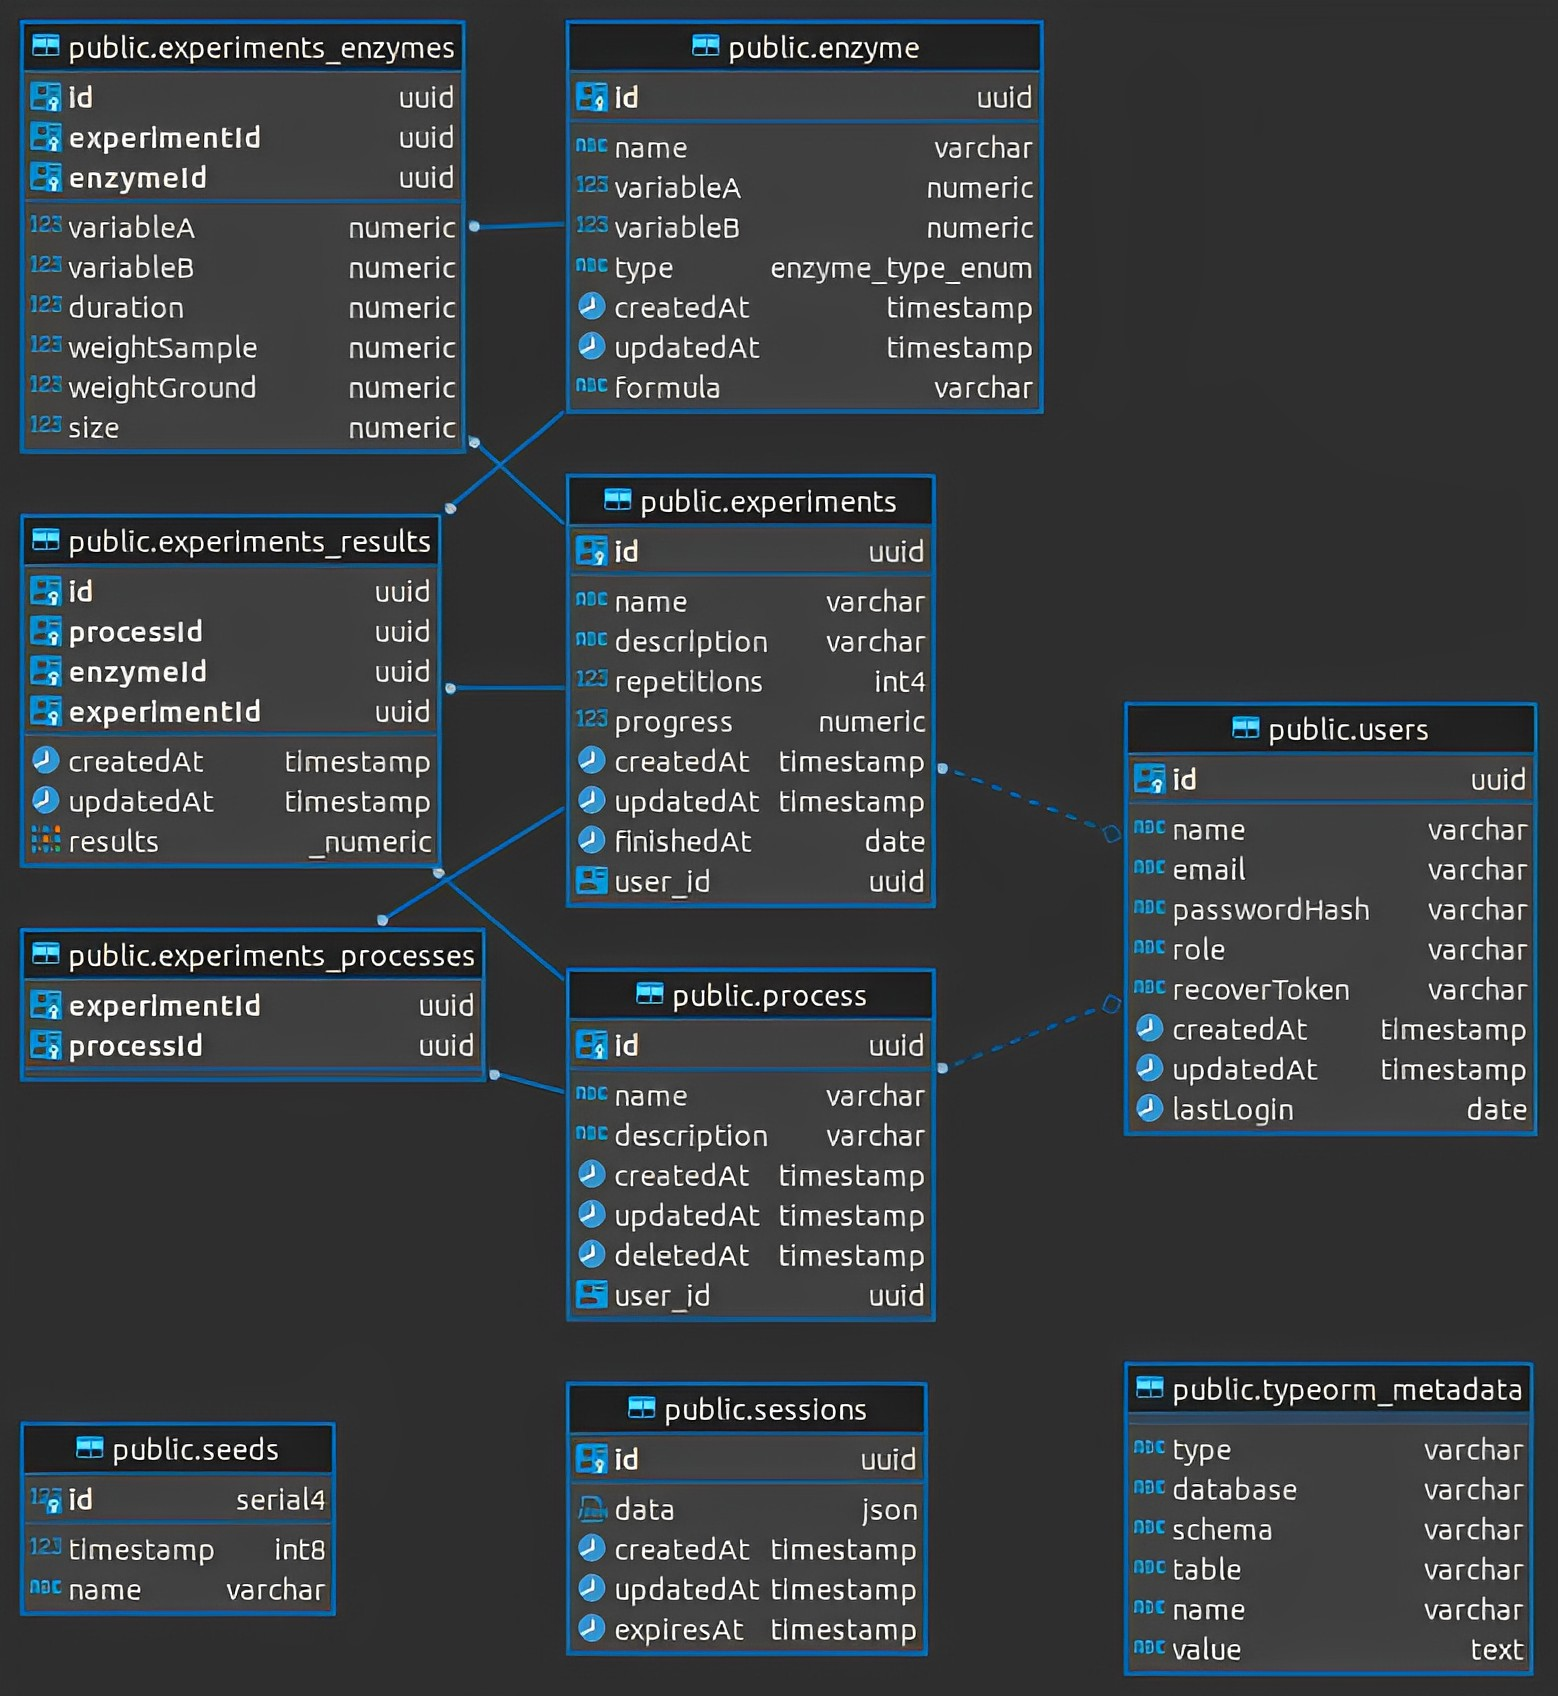
\includegraphics[width=\columnwidth]{images/er.jpg}
  \caption{Diagrama de Entidade-Relacionamento do Enzitech}
  \acsfont{Fonte: DBeaver\footref{dbeaver}}
  \label{fig:der}
\end{figure}

Através da modelagem com o diagrama ER, é possível criar um modelo lógico para o banco de dados, abstraindo as características específicas da tecnologia a ser utilizada, facilitando a implementação do modelo físico do banco de dados. Na \figref{fig:der} é possível ver como ficou o diagrama ER do Enzitech, após consulta do mesmo no software para gerenciamento de banco de dados, DBeaver\footnote{\label{dbeaver}DBeaver: \url{https://dbeaver.com/docs/wiki/ER-Diagrams/}}.

\section{Arquitetura do sistema}\label{sec:arquitetura}
A Arquitetura do sistema por completo pode ser considerada uma arquitetura híbrida, pois a mesma utiliza princípios de quatro padrões arquiteturais, sendo eles:

\begin{enumerate}
   \item \ac{mvvm}: Arquitetura de \ac{ui} para evitar o acoplamento das camadas de \acp{ui} das de negócios;
   \item Cliente-Servidor: Arquitetura para comunicação entre o \textit{front-end} e o \textit{back-end}/\ac{api};
   \item Monolítico: Arquitetura em que todo o sistema é desenvolvido em um único bloco de código, uma só instancia que gerencia todos os estados da aplicação, sem divisão clara de módulos ou serviços;
   \item Arquitetura Limpa: Arquitetura com o foco em promover a implementação de sistemas que favorecem reusabilidade de código, coesão, independência de tecnologia e testabilidade;
 \end{enumerate}

O \textit{back-end} gerencia todas as solicitações feitas pelo \ac{app}, manipulando os dados por meio de operações \ac{crud} em uma instância de banco de dados Postgresql\footnote{\label{postgresql}Postgresql: \url{https://www.postgresql.org/}}.

A comunicação entre o cliente e o \textit{back-end} é estabelecida por meio de requisições \ac{http}, que são processadas pela \ac{api} do \textit{back-end} e resultam em respostas adequadas, formatadas em \ac{json}. O cliente, por sua vez, é responsável por exibir as informações ao usuário final e coletar as interações do usuário para posteriormente enviar ao \textit{back-end}.

A arquitetura adotada busca garantir a escalabilidade e a segurança do sistema, bem como a facilidade de manutenção. O \textit{back-end} é projetado seguindo os padrões RESTful (capacidade de determinado sistema aplicar os princípios de \ac{rest}), o que permite a integração com outros sistemas e garante a interoperabilidade. O uso do Postgresql\footref{postgresql} como banco de dados permite a manipulação de grandes volumes de dados e garante a consistência dos dados armazenados. Além disso, a utilização de boas práticas de segurança, como a autenticação e autorização de usuários, garante que apenas usuários autorizados possam acessar os dados do sistema.

Por fim, a arquitetura do sistema é projetada para atender às necessidades do cliente \textit{mobile}, oferecendo uma experiência de usuário agradável e uma interface responsiva, que garante o bom desempenho do \ac{app}. A seguir, serão destrinchadas as arquiteturas do aplicativo e da infraestrutura do sistema.

\begin{figure}[H]
\centering
  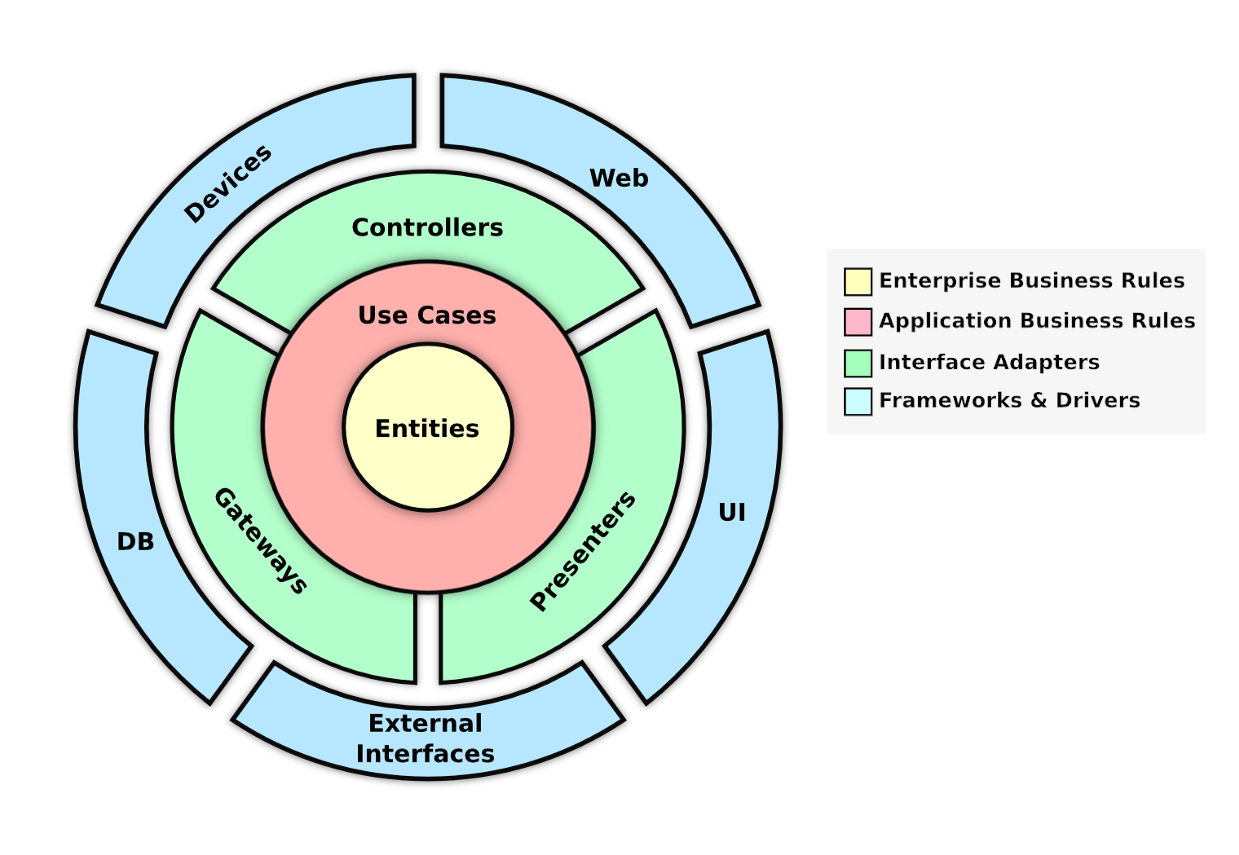
\includegraphics[width=0.9\columnwidth]{images/clean_dart.png}
  \caption{Camadas de uma Arquitetura Limpa}
  \acsfont{Fontes: \cite{martin2018arquitetura} e \cite{flutterando_clean_dart}}
  \label{fig:clean_dart}
\end{figure}

Como apontado por \cite{martin2018arquitetura}, uma arquitetura deve conter pelo menos estas quatro camadas principais e independentes para ser considerada “limpa”:
\begin{itemize}
   \item \textbf{Regras de Negócio Corporativas:} As entidades são modelos de dados que representam as regras de negócio mais importantes de um sistema e estão no topo das camadas. Elas devem ser puras, não conhecendo nenhuma outra camada, mas são conhecidas pelas outras camadas;
   \item \textbf{Regras de Negócio da Aplicação:} Os casos de uso representam as ações que um usuário pode fazer na aplicação. Os casos de uso conhecem apenas as entidades, não sabendo sobre as implementações de camadas de baixo nível. Se precisarem acessar uma camada superior, devem fazê-lo por meio de contratos definidos por interfaces, seguindo o Princípio de Inversão de Dependências do SOLID;
   \item \textbf{Adaptadores de Interface:} Camada responsável por auxiliar as Regras de Negócios, convertendo os dados externos em um formato que atenda aos contratos de interface definidos por ela;
   \item \textbf{Frameworks \& Drivers (Externos):} Abstrações feitas para aumentar a facilidade da conexão dos artefatos externos como um banco de dados, protocolo de requisições web ou uma interface gráfica, facilitando a troca sem alterar o comportamento do sistema;
 \end{itemize}

 Desta forma, a aplicação da arquitetura limpa sugerida no Flutter/Dart pela comunidade \cite{flutterando_clean_dart} segue o fluxo da \figref{fig:clean_dart2} a seguir:

\begin{figure}[H]
\centering
  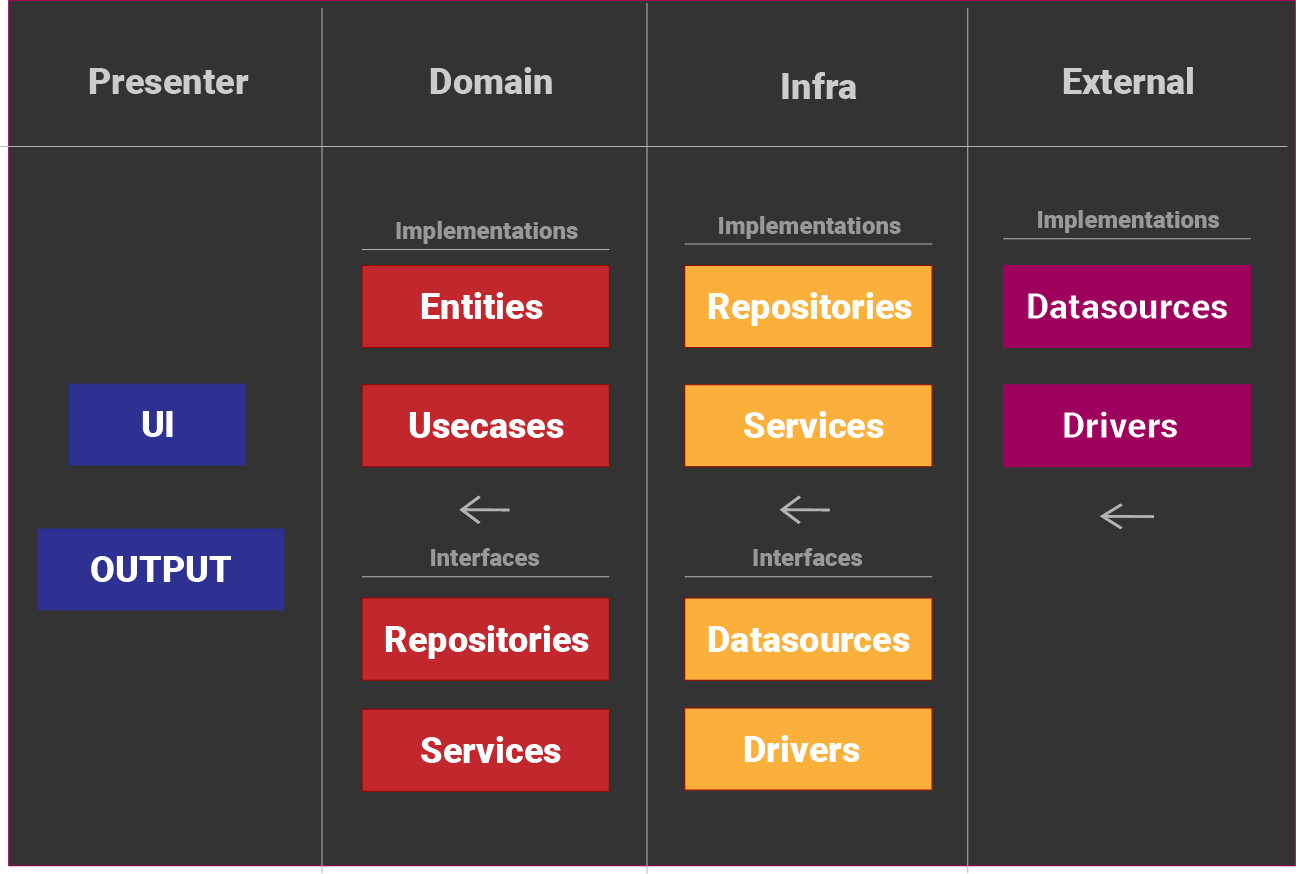
\includegraphics[width=0.8\columnwidth]{images/clean_dart2.png}
  \caption{Sugestão da estrutura das camadas de uma Arquitetura Limpa no Flutter}
  \acsfont{Fonte: \cite{flutterando_clean_dart}}
  \label{fig:clean_dart2}
\end{figure}

Para aplicação \textit{mobile} desenvolvida, esta proposta de arquitetura foi abstraída em três camadas maiores, mas seguindo o padrão e as peculiaridades da proposta acima, sendo assim, a arquitetura seguiu com as seguintes camadas:

\begin{itemize}
   \item \textbf{Presentation:} Camada responsável por declarar as entradas, saídas e interações da aplicação. onde ficarão os \textit{Widgets}, \textit{Pages}, \textit{ViewModels} das respectivas \textit{Pages} e também a Gerência de Estado;
   \item \textbf{Domain:} Camada que hospeda as Entidades (Regras de Negócio Corporativa), os Casos de Uso (Regras de Negócio da Aplicação) e os contratos dos Repositórios (a responsabilidade de implementação desse objeto é repassado para outra camada mais baixa), fazendo com que esta camada seja responsável apenas pela execução da lógica de negócio, não havendo implementações de outros objetos fora da mesma;
   \item \textbf{Data:} Camada que dá suporte à camada Domain, implementando suas interfaces. Para isso, adapta os dados externos para que possa cumprir os contratos do domínio. Nesta camada é possível implementar alguma interface de um Repositório ou Serviço que pode ou não depender de dados externos como uma \ac{api} ou acesso a algum \textit{Hardware} como por exemplo GPS. Para que o Repositório possa processar e adaptar os dados externos foram criados contratos para esses serviços visando passar a responsabilidade de implementação para a camada mais baixa dessa arquitetura: o DataSource, esta camada interna em Data permite acessar um dado externo, como a \ac{api} do Enzitech ou um Cache Local usando \textit{SharedPrefs} por exemplo, como há uma redução de camadas, é aqui onde os acessos externos são implementados seguindo o mesmo padrão de contratos como acontece entre Domain e Data, realizado na aplicação fora das camadas de \textit{features} que possuem a mesma estrutura, assim, ainda preservando a separação de responsabilidades e tornando os pacotes externos desacoplados da nossa aplicação, como deve ser na arquitetura limpa;
 \end{itemize}

Para concluir, um exemplo abaixo da arquitetura de toda a infraestrutura do Enzitech:

\begin{figure}[H]
\centering
  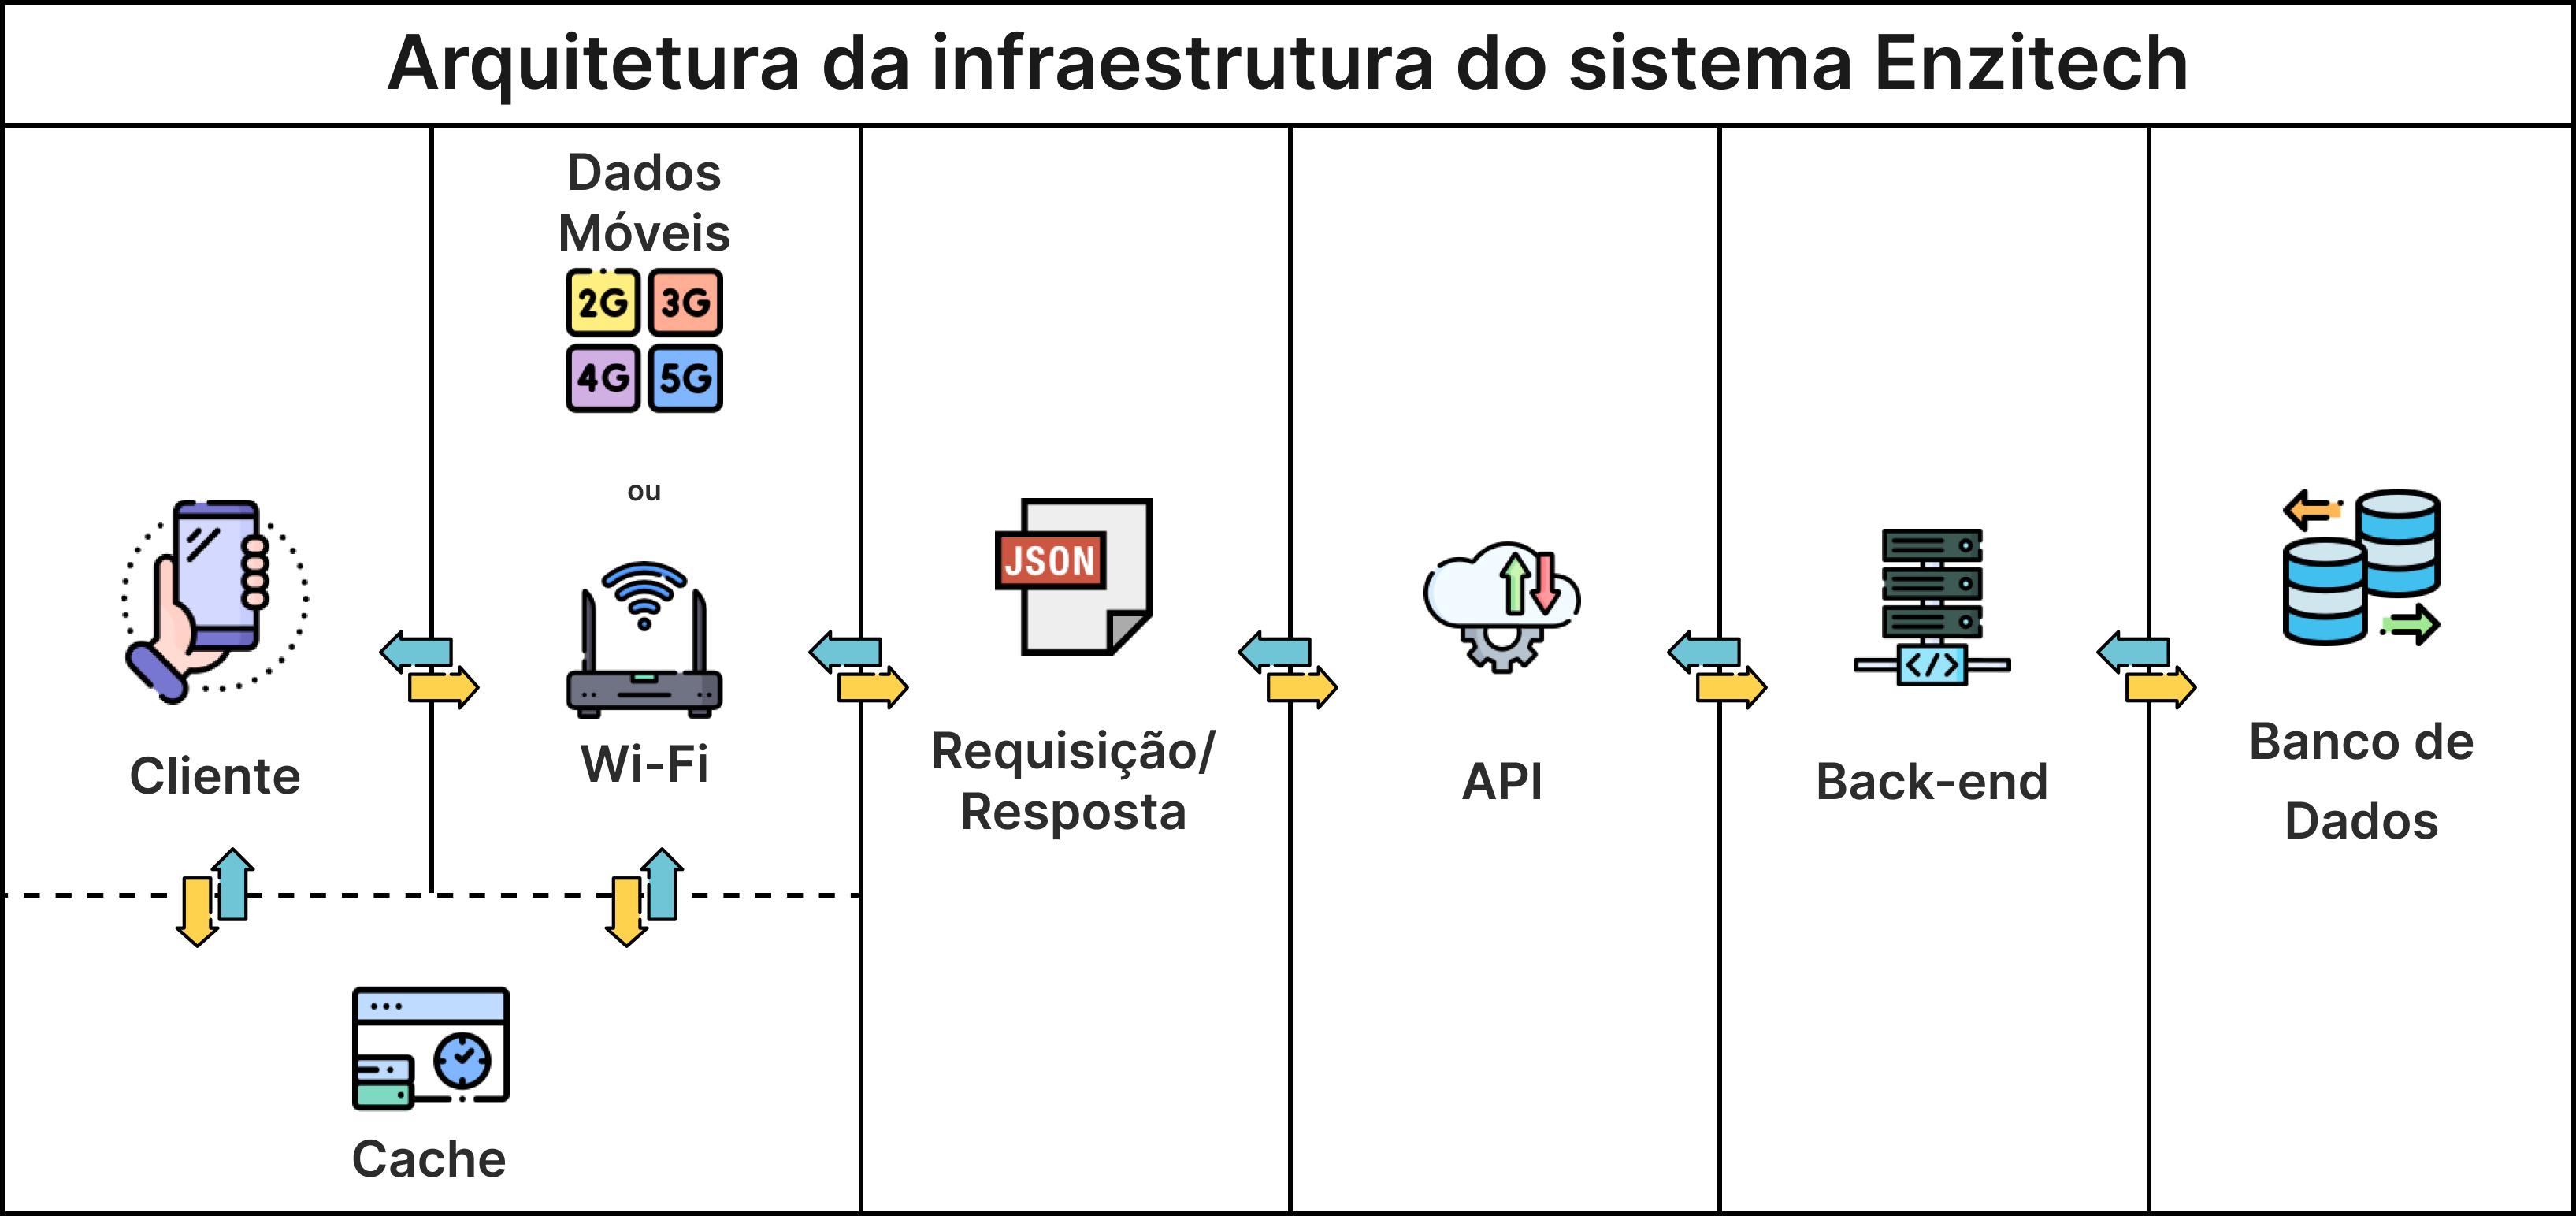
\includegraphics[width=\columnwidth]{images/arquitetura_enzitech.png}
  \caption{Arquitetura simplificada da infraestrutura do Enzitech}
  % \acsfont{Fonte: DBeaver\footref{dbeaver}}
  \label{fig:arquitetura_enzitech}
\end{figure}

A arquitetura da aplicação ilustrada na \figref{fig:arquitetura_enzitech} foi desenvolvida baseado na proposta de arquitetura de \cite{martin2018arquitetura}, também do seu livro sobre \nameref{sec:arquitetura_limpa}, arquitetura esta que é separada em camadas, com o objetivo de simplificar a codificação, possibilitando sua manutenção e atualização de forma prática, reduzindo a dependência do código. Com base nesta arquitetura descrita, é possível destacar alguns pontos adicionais:

\begin{itemize}
   \item O aplicativo \textit{mobile} é responsável por fornecer uma interface de usuário amigável e eficiente para interação com o sistema. Isso inclui a exibição de informações, a coleta de dados de entrada e a navegação entre diferentes telas e funcionalidades;
   % \item A \ac{api} do \textit{back-end} é projetada seguindo os padrões RESTful, que define um conjunto de práticas recomendadas para a criação de serviços web. Isso inclui o uso de métodos \ac{http} (GET, POST, PUT, DELETE) para manipulação de recursos, a definição de \acp{url} consistentes para acesso aos recursos e o uso de formatos de dados padronizados no formato \ac{json} para comunicação entre o cliente e o servidor;
   % \item O \textit{back-end} é responsável por realizar as operações de \ac{crud} no banco de dados, garantindo a integridade dos dados armazenados. Isso inclui a validação de dados de entrada, a realização de consultas e atualizações no banco de dados e a manipulação de erros e exceções;
   % \item A utilização de boas práticas de segurança é essencial para garantir a integridade e a confidencialidade dos dados do sistema. Isso inclui a implementação de autenticação e autorização de usuários, o uso de criptografia para proteção de dados sensíveis, a realização de backups periódicos do banco de dados e a adoção de medidas de prevenção contra ataques e invasões;
   \item A escalabilidade do sistema é uma preocupação importante, uma vez que o número de usuários e a quantidade de dados podem crescer significativamente ao longo do tempo. Para garantir a escalabilidade, é possível adotar soluções como a utilização de servidores em nuvem, a implementação de técnicas de cache e a otimização de consultas no banco de dados;
   \item A arquitetura do sistema foi projetada para facilitar a manutenção e o desenvolvimento de novas funcionalidades. Isso inclui a utilização de padrões de codificação consistentes, a documentação adequada do código-fonte e a realização de testes unitários e de integração para garantir a qualidade do software;
 \end{itemize}

\section{Testes}
Antes de ser implantado, o aplicativo foi testado em suas \textit{releases} pela equipe interna do Enzitech, além disso, no desenvolvimento, foram utilizados técnicas de teste, como integração, aceitação e de unidade, no fim deste arquivo, no capítulo \nameref{ch:testes} é possível verificar esta etapa.

Dentro da seção "\nameref{code:teste-unidade-enzima}", é possível ver um exemplo de teste de unidade escrito na linguagem de programação Dart, usando o \textit{framework} de testes padrão do Flutter, o teste é uma função anônima (sem nome) que verifica se a instância da classe \textit{EnzymeEntity} não é nula. O nome do teste é \textit{"Should not return null on Enzyme entity"}.

Dentro do corpo da função, é criada uma nova instância da classe \textit{EnzymeEntity} e atribuída à variável \textit{enzyme}. O construtor da classe \textit{EnzymeEntity} é chamado com argumentos específicos para inicializar as propriedades da instância. Em seguida, é usada a função \textit{expect()} do \textit{framework} de teste para verificar se a instância da classe \textit{EnzymeEntity} criada anteriormente não é nula. Se a expectativa for cumprida, o teste passa. Caso contrário, o teste falha.

Este teste serve como uma verificação básica para garantir que a classe \textit{EnzymeEntity} esteja sendo inicializada corretamente e não esteja retornando um valor nulo.

\section{Implantação}
O \textit{back-end} e o banco de dados do sistema Enzitech foram implantados na infraestrutura da \ac{ufape}, utilizando-se dos recursos de processamento e armazenamento disponibilizados pela instituição. A \ac{api} desenvolvida para o projeto foi disponibilizada através de uma rota pública, permitindo o acesso aos dados e funcionalidades do sistema a partir do aplicativo desenvolvido para os usuários finais. A escolha pela hospedagem na infraestrutura da \ac{ufape} teve como objetivo garantir a segurança, estabilidade e escalabilidade da aplicação, além de possibilitar a utilização de recursos computacionais locais e adequados para as necessidades do projeto.

O aplicativo móvel foi projetado para alterar facilmente entre os ambientes de desenvolvimento, teste ou produção, desta forma, em sua versão final, o \ac{app} foi distribuído internamente via \textit{Firebase App Distribution}, porém sendo possível também a sua publicação na \textit{Google Play Store}, loja de \acp{app} do Android. 
